\documentclass[UTF8,  zihao=-4]{ctexart}

% 页面与字体
\usepackage[a4paper,  margin=2.7cm]{geometry}
\usepackage{setspace}
\setstretch{1.28}
\setlength{\parindent}{2em}
\setlength{\parskip}{0.25em}

\usepackage{amsmath,  amssymb,  mathtools}
\usepackage{geometry}
\usepackage{xcolor}
\usepackage{graphicx}
\usepackage{pdfpages}
\usepackage{xurl}
\usepackage{caption}
\usepackage{listings}
\usepackage{booktabs}
\usepackage{array}
\usepackage{algorithm}
\usepackage{algpseudocode}
\usepackage{setspace}
\usepackage{indentfirst}
\usepackage[most]{tcolorbox}

\setstretch{1.15}
\setlength{\parindent}{2em}
\setlength{\parskip}{0pt}
\setlength{\textfloatsep}{7pt plus 2pt minus 2pt}
\setlength{\floatsep}{6pt plus 2pt minus 1pt}
\setlength{\intextsep}{7pt plus 2pt minus 2pt}
\setlength{\abovecaptionskip}{3pt}
\setlength{\belowcaptionskip}{2pt}
\captionsetup{aboveskip=3pt,  belowskip=2pt}
\captionsetup[figure]{aboveskip=3pt,  belowskip=2pt}
\captionsetup[table]{aboveskip=3pt,  belowskip=2pt}
\captionsetup[algorithm]{aboveskip=3pt,  belowskip=2pt}
\renewcommand{\topfraction}{0.95}
\renewcommand{\bottomfraction}{0.85}
\renewcommand{\textfraction}{0.05}
\renewcommand{\floatpagefraction}{0.70}
\makeatletter
\setlength{\@fptop}{0pt}
\setlength{\@fpsep}{7pt plus 2pt minus 1pt}
\setlength{\@fpbot}{0pt plus 1fil}
\makeatother

\renewcommand{\tablename}{表}
\renewcommand{\figurename}{图}
\renewcommand{\refname}{参考文献}
\floatname{algorithm}{算法}
\newenvironment{breakablealgorithm}[2]{%
    \refstepcounter{algorithm}%
    \addcontentsline{loa}{algorithm}{\protect\numberline{\thealgorithm}{#1}}%
    \begin{tcolorbox}[
        enhanced, 
        breakable, 
        colback=white, 
        colbacktitle=white, 
        frame hidden, 
        boxrule=0pt, 
        arc=0pt, 
        outer arc=0pt, 
        left=0pt, 
        right=0pt, 
        top=2pt, 
        bottom=2pt, 
        before skip=3pt, 
        after skip=3pt, 
        overlay unbroken={
            \draw[line width=0.4pt] (frame.north west) -- (frame.north east);
            \draw[line width=0.4pt] (frame.south west) -- (frame.south east);
        }, 
        overlay first={
            \draw[line width=0.4pt] (frame.north west) -- (frame.north east);
            \draw[line width=0.4pt] (frame.south west) -- (frame.south east);
        }, 
        overlay middle={
            \draw[line width=0.4pt] (frame.north west) -- (frame.north east);
            \draw[line width=0.4pt] (frame.south west) -- (frame.south east);
        }, 
        overlay last={
            \draw[line width=0.4pt] (frame.north west) -- (frame.north east);
            \draw[line width=0.4pt] (frame.south west) -- (frame.south east);
        }
    ]
    \noindent\small\textbf{算法 \thealgorithm: #1}\label{#2}\par
    \vspace{0.15em}\hrule\vspace{0.25em}
    \raggedright\footnotesize
}{%
    \end{tcolorbox}%
}

\DeclareMathOperator{\Var}{Var}
\newcommand{\E}{\mathbb{E}}
\newcommand{\Prob}{\mathbb{P}}

% 页眉页脚
\usepackage{fancyhdr}
\pagestyle{fancy}
\fancyhf{}
\cfoot{\thepage}
\renewcommand{\headrulewidth}{0pt}
\renewcommand{\footrulewidth}{0pt}
\setcounter{secnumdepth}{4}
\setcounter{tocdepth}{4}
\usepackage{titlesec}

\titleformat{\paragraph}
  {\normalfont\normalsize\bfseries}
  {\theparagraph}
  {1em}
  {}

\titlespacing*{\paragraph}
  {0pt}
  {1.0ex plus 0.2ex minus 0.2ex}
  {0.8ex}
\usepackage[hidelinks, linktoc=all]{hyperref}
\lstset{
    language=Python,  
    basicstyle=\ttfamily\small,  
    breaklines=true,  
    frame=single,  
    numbers=left,  
    numberstyle=\tiny,  
    showstringspaces=false,  
    columns=fullflexible,  
    keywordstyle=\bfseries
}
\title{神经网络作业}
\author{林立康\quad 计算数学\quad 25210180078}

\begin{document}

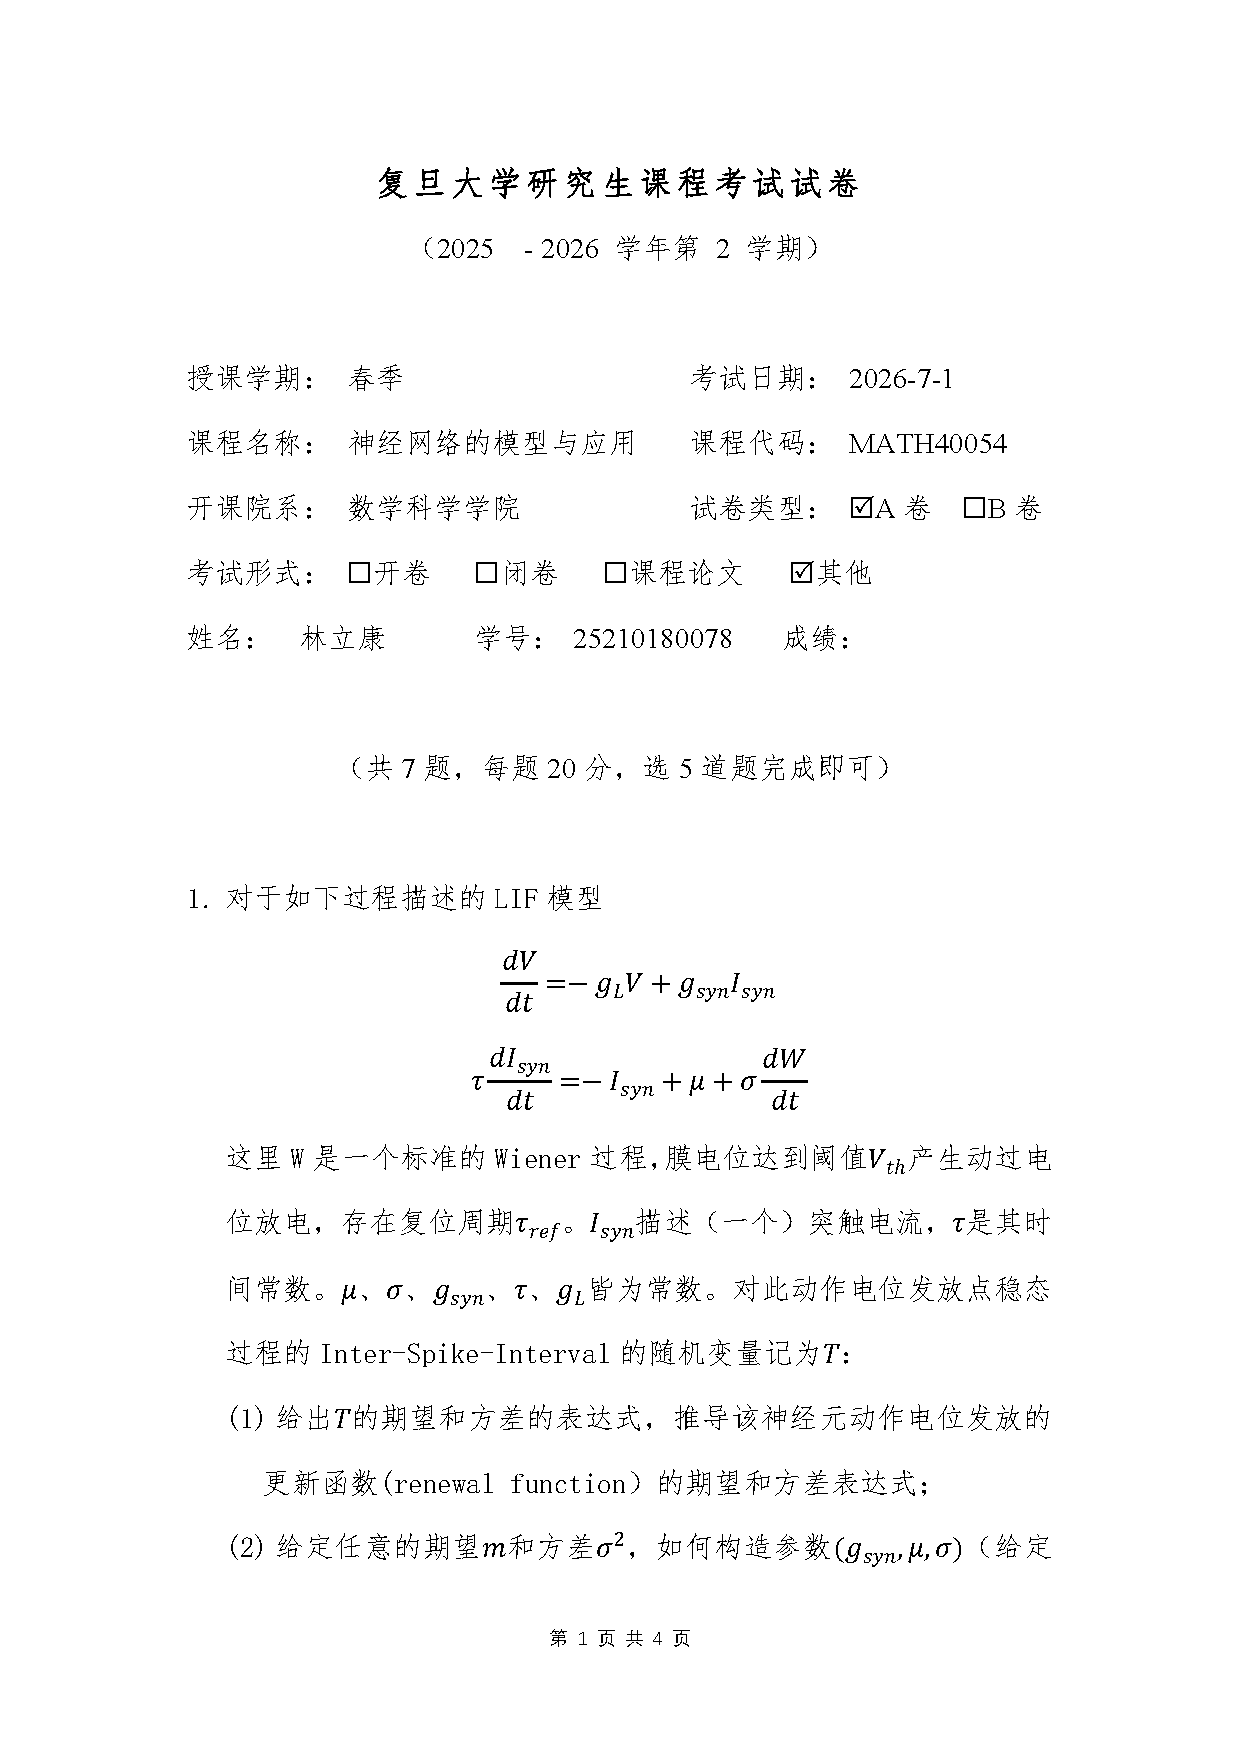
\includepdf[pages=-]{试卷.pdf}

\clearpage
\begin{titlepage}
\pagestyle{empty}
\begin{center}
\vspace*{0.7cm}

{\zihao{2}\heiti 《神经网络的模型与应用》期终考试答题部分\par}

\vspace{0.6cm}

{\zihao{4} 林立康\quad 计算数学\quad 25210180078\par}

\vspace{0.6cm}

{\zihao{4}\heiti 摘\quad 要\par}
\end{center}

\vspace{0.25em}

\begingroup
\zihao{-4}
\setstretch{1.24}
\setlength{\parindent}{2em}
\setlength{\parskip}{0.18em}
选取了第1、4、5、6、7题进行解答. 相关代码参见附件或 \url{https://github.com/LiHuaGz/NN_exam.git}.

第1题.对于第一小问(原题第一小问的第二点要求的是更新函数$M(t)=\mathbb{E}[N(t)]$的期望与方差,  然而$M(t)$已经是某个随机变量的期望了,  笔者猜测原题是笔误,  因此在解答中第一小问求解的是$T$和\(N(t)\)的期望与方差表达式. 其中,  脉冲间隔序列为$T_i, S_n=T_1+T_2+\cdots+T_n,  S_0=0,  N(t)=\max\{n: S_n\leq t\}$),  首先将一次完整的 Inter-Spike-Interval 表示为不应期与首次过阈时间之和, 并利用二维 Markov 扩散过程的生成元和 backward Kolmogorov 方程给出首次过阈时间一阶矩, 二阶矩及方差的表达式;随后将动作电位发放序列视为更新过程, 推导出更新函数 \(M(t)=\mathbb E[N(t)]\) 以及发放计数 \(N(t)\) 方差的卷积级数表达式,  具体表达式见\ref{sec1:solve}.对于第二小问, 针对给定目标均值和方差, 利用无噪声轨道确定有效输入均值参数, 再通过小噪声展开构造有效噪声强度, 从而得到 \((g_{\mathrm{syn}}, \mu, \sigma_I)\) 的参数选取方法. Monte Carlo 数值实验表明, 所构造参数下模拟得到的脉冲间隔均值与目标均值接近, 方差也与目标值基本吻合, 验证了该近似构造的有效性.

第4题.首先, 根据条件独立泊松过程假设, 说明发放时间点中关于刺激方向 \(s\) 的信息可以归约为各神经元在观测时间窗内的发放计数, 并据此建立联合似然函数和对数似然函数. 其次, 由于有限样本下严格 MVUB 估计量难以写成简单解析形式, 本文采用极大似然估计作为渐近意义下的近似 MVUB 解, 并推导其一阶最优条件,  Fisher 信息和 Cramér--Rao 下界.理论分析表明, 在观测时间窗较大时,  MLE 近似无偏且方差接近 Fisher 信息倒数, 因此其均方误差可由 CRLB 近似刻画. 最后, 数值模拟进一步显示, 随着观测时间增加, 经验 MSE 逐渐下降并接近 CRLB, 估计偏差趋近于零, 说明该估计方法在较大样本下具有良好的渐近性.

第5题. 针对附件音频数据进行盲源分离, 并比较 FastICA 与 AMUSE 两种算法的分离效果.首先建立线性混合模型 \(X=AS\), 并通过去均值, 白化等预处理将问题转化为白化空间中的正交分离问题. FastICA 利用独立源信号的非高斯性, 通过 \(\tanh\) 非线性函数和对称去相关迭代估计分离矩阵; AMUSE 则利用源信号的时间相关结构, 通过延迟协方差矩阵的近似对角化完成分离.由于没有真实源信号作为参考, 实验采用平均绝对相关系数、归一化互信息、时间协方差非对角项和平均绝对超额峰度等无参考指标评价质量.结果显示, 两种算法均显著降低了分量间统计依赖并提高了非高斯性,  FastICA 和 AMUSE 的分离效果整体接近, 其中 AMUSE 在时间协方差非对角项和互信息指标上略优.

第6题. 在 MNIST 手写数字分类任务上比较带动量 SGD 与阻尼小批量自然梯度法的训练表现, 实验采用相同的全连接层(网络结构为\(784\to128\to64\to10\)), 隐藏层使用 ReLU, 输出层使用 softmax 交叉熵损失.由于完整 Fisher 信息矩阵存储代价过高, 自然梯度部分使用 KL 散度 Hessian 的 Fisher 向量积, 并通过共轭梯度法近似求解 \((F+\lambda I)d=\nabla_\theta L\), 再进行参数更新. 实验在本地CPU上进行. 数值结果表明, 两种方法都能稳定收敛, 但在本次超参数设置下,  SGD 的收敛速度和最终测试准确率略优于自然梯度; SGD 第 5 轮测试准确率达到 \(97.41\%\), 自然梯度达到 \(96.38\%\).这说明阻尼自然梯度实现能够在不显式存储 Fisher 矩阵的情况下完成训练, 但其效果受阻尼系数、学习率、共轭梯度迭代次数和裁剪策略影响较大.

第7题. 利用强化学习思想求解迷宫最短路径搜索问题.程序首先从迷宫图像中自动识别黄色起点, 迷宫边界, 网格大小, 墙体和可通行区域, 并将图像转化为离散状态空间;每个可通行格子作为一个状态, 动作为上, 下, 左, 右四个方向.路径规划部分采用 Bellman 最优性更新, 设置到达目标后的价值为 \(0\), 其余每移动一步奖励为 \(-1\), 折扣因子取 \(\gamma=1\), 从而使最优价值函数等价于到目标点最短距离的相反数.若目标点不可达, 程序直接给出不可达判断;若目标可达, 则沿价值最大的相邻格贪心回溯得到最短路径, 并将路径绘制在原始迷宫图上. 实验随机选取了两组终点(亦可手动选取), 并设计了交互式界面. 实验表明该方法能够在不同目标位置下避开墙体并得到从起点到终点的可行最短路线.

\vspace{1.2em}

\noindent
{\heiti 关键词:} 随机 LIF 模型, 更新过程, 泊松发放模型, FastICA, AMUSE, 自然梯度, Bellman 迭代, 迷宫路径规划
\par
\endgroup

\end{titlepage}

\clearpage
\pagestyle{empty}
\tableofcontents
\clearpage
\pagestyle{fancy}
\pagenumbering{arabic}
\setcounter{page}{1}

\section{第1题}
\subsection{第1小问}
\subsubsection{问题重述与记号约定}
考虑该随机 LIF 模型产生的动作电位发放序列:
\begin{equation}
\label{eq:q1_LIF}
\begin{aligned}
\frac{dV}{dt} &= -g_L V + g_{\mathrm{syn}} I_{\mathrm{syn}},  \\
\tau \frac{d I_{\mathrm{syn}}}{dt}
&= -I_{\mathrm{syn}} + \mu + \sigma \frac{dW}{dt}.
\end{aligned}
\end{equation}
设相邻两次动作电位之间的时间间隔为 \(T\), 并假设每次放电后神经元完成复位, 系统重新开始下一次积分--发放过程.脉冲间隔序列 \(T_1,  T_2, \ldots\) 可视为独立同分布随机变量, 且设 \(T_k\sim T\).

定义第 \(n\) 次动作电位发放时刻为
\[
S_n=T_1+T_2+\cdots+T_n, \qquad S_0=0.
\]
于是, 到时刻 \(t\) 为止的动作电位发放次数为
$
N(t)=\max\{n: S_n\leq t\}, 
$
其更新函数定义为
$
M(t)=\mathbb{E}[N(t)].
$

\textbf{注:} \(M(t)\) 已经是 \(N(t)\) 的数学期望, 而不是随机变量;有非平凡方差的是\(N(t)\), 而不是 \(M(t)\),  笔者猜测原题目中有笔误.下面推导$T$和\(N(t)\)的期望与方差表达式.

\subsubsection{问题求解}
\label{sec1:solve}
\paragraph{\texorpdfstring{\(T\)的期望与方差}{T 的期望与方差}}

设神经元放电后膜电位被复位到
\(V_r\), 并经过 \(\tau_{\mathrm{ref}}\) 后重新开始积分.令
$\theta=
\inf\{t>0: V(t)\geq V_{th} \}.
$
因此, 一个完整的脉冲间隔可写为
$
T=\tau_{\mathrm{ref}}+\theta .
$

由题设模型可知, 
\[
dV
=
\left(-g_LV+g_{\mathrm{syn}}I_{\mathrm{syn}}\right)dt, 
\]
\[
dI_{\mathrm{syn}}
=
\frac{\mu-I_{\mathrm{syn}}}{\tau}dt
+
\frac{\sigma}{\tau}dW_t .
\]
因此\((V(t),  I_{\mathrm{syn}}(t))\) 构成二维 Markov 扩散过程.记
\[
u_1(v,  i)
=
\mathbb{E}_{v,  i}[\theta], 
\qquad
u_2(v,  i)
=
\mathbb{E}_{v,  i}[\theta^2], 
\]
其中下标 \((v,  i)\) 表示初始条件为
$V(0)=v,  I_{\mathrm{syn}}(0)=i.
$

该二维过程的生成元为
\[
\mathcal{L}
=
\left(-g_Lv+g_{\mathrm{syn}}i\right)\frac{\partial}{\partial v}
+
\frac{\mu-i}{\tau}\frac{\partial}{\partial i}
+
\frac{\sigma^2}{2\tau^2}\frac{\partial^2}{\partial i^2}.
\]
根据首次通过时间矩的 backward Kolmogorov 方程, \(u_1(v,  i)\)
满足
\[
\mathcal{L}u_1(v,  i)=-1, 
\qquad v<V_{th}, 
\]
\(u_2(v,  i)\) 满足
\[
\mathcal{L}u_2(v,  i)=-2u_1(v,  i), 
\qquad v<V_{th}.
\]
相应的吸收边界条件为
$
u_1(V_{th},  i)=0, 
u_2(V_{th},  i)=0.
$

(1) 若复位后突触电流初值固定为 \(I_{\mathrm{syn}}(0)=i\), 则
\[
\mathbb{E}[T\mid I_{\mathrm{syn}}(0)=i]
=
\tau_{\mathrm{ref}}+u_1(V_r,  i), 
\]
并且
\[
\operatorname{Var}(T\mid I_{\mathrm{syn}}(0)=i)
=
u_2(V_r,  i)-u_1^2(V_r,  i).
\]

(2) 若复位后 \(I_{\mathrm{syn}}(0)\) 不是固定值, 而是服从某个分布
\(\rho(i)\), 则需要对初始突触电流再取平均.此时
\[
\mathbb{E}[T]
=
\tau_{\mathrm{ref}}
+
\int_{-\infty}^{+\infty}u_1(V_r,  i)\rho(i)\,  di, 
\]
且
\[
\operatorname{Var}(T)
=
\int_{-\infty}^{+\infty}u_2(V_r,  i)\rho(i)\,  di
-
\left(
\int_{-\infty}^{+\infty}u_1(V_r,  i)\rho(i)\,  di
\right)^2.
\]

(3) 特别地, 若假设复位后突触电流已经处于 OU 过程的稳态分布, 则
$
I_{\mathrm{syn}}(0)
\sim
\mathcal{N}
\left(
\mu, \frac{\sigma^2}{2\tau}
\right), 
$
因此
$
\rho(i)
=
\sqrt{\frac{\tau}{\pi\sigma^2}}
\exp\left\{
-\frac{\tau(i-\mu)^2}{\sigma^2}
\right\}.
$
于是 \(T\) 的期望与方差可分别写为
\[
\mathbb{E}[T]
=
\tau_{\mathrm{ref}}
+
\int_{-\infty}^{+\infty}u_1(V_r,  i)
\sqrt{\frac{\tau}{\pi\sigma^2}}
\exp\left\{
-\frac{\tau(i-\mu)^2}{\sigma^2}
\right\}
\,  di, 
\]
以及
\[
\begin{aligned}
\operatorname{Var}(T)
&=
\int_{-\infty}^{+\infty}u_2(V_r,  i)
\sqrt{\frac{\tau}{\pi\sigma^2}}
\exp\left\{
-\frac{\tau(i-\mu)^2}{\sigma^2}
\right\}
\,  di
\\
&\quad
-
\left[
\int_{-\infty}^{+\infty}u_1(V_r,  i)
\sqrt{\frac{\tau}{\pi\sigma^2}}
\exp\left\{
-\frac{\tau(i-\mu)^2}{\sigma^2}
\right\}
\,  di
\right]^2.
\end{aligned}
\]


\paragraph{\texorpdfstring{\(N(t)\)的期望与方差}{N(t) 的期望与方差}}
\textbf{(1) \(N(t)\)的期望}

令 \(F_T(t)=\mathbb{P}(T\leq t)\) 表示 ISI 随机变量 \(T\) 的分布函数.由于 \(S_n=T_1+\cdots+T_n\), 所以 \(S_n\) 的分布函数为 \(F_T\) 的 \(n\) 重卷积, 记为 \(F_T^{*n}(t)\), 即
$
F_T^{*n}(t)=\mathbb{P}(S_n\leq t).
$
注意到事件 \(\{N(t)\geq n\}\) 与事件 \(\{S_n\leq t\}\) 等价, 因此有
\[
\mathbb{P}(N(t)\geq n)=\mathbb{P}(S_n\leq t)=F_T^{*n}(t).
\]
由非负整数值随机变量的尾和公式可得
\[
M(t)=\mathbb{E}[N(t)]
=
\sum_{n=1}^{\infty}\mathbb{P}(N(t)\geq n)
=
\sum_{n=1}^{\infty}F_T^{*n}(t).
\]

\textbf{(2) \(N(t)\)的方差}

由于对任意非负整数 \(k\), 有 \(k^2=\sum_{n=1}^{k}(2n-1)\), 因此
\[
N(t)^2
=
\sum_{n=1}^{\infty}(2n-1)\mathbf{1}_{\{N(t)\geq n\}}.
\]
两边取期望, 得到
\[
\mathbb{E}[N(t)^2]
=
\sum_{n=1}^{\infty}(2n-1)\mathbb{P}(N(t)\geq n)
=
\sum_{n=1}^{\infty}(2n-1)F_T^{*n}(t).
\]
因此, 发放计数过程 \(N(t)\) 的方差为
\[
\operatorname{Var}(N(t))
=
\sum_{n=1}^{\infty}(2n-1)F_T^{*n}(t)
-
\left(
\sum_{n=1}^{\infty}F_T^{*n}(t)
\right)^2.
\]

\textbf{注: }上述表达式依赖于 \(T\) 的分布 \(F_T\). 若仅已知 \(\mathbb{E}[T]\) 与 \(\operatorname{Var}(T)\), 则只能给出近似值(\(t\) 足够大):
\[
M(t)=\mathbb{E}[N(t)]\approx \frac{t}{\mathbb{E}[T]}
, 
\qquad
\operatorname{Var}(N(t))\approx \frac{\operatorname{Var}(T)}{(\mathbb{E}[T])^3}t
.
\]

\subsection{第2小问}
\subsubsection{理论推导}
为避免记号混淆,  本节沿用第1小问的记号: \(T\) 表示完整脉冲间隔,  \(\theta\) 表示膜电位从复位值 \(V_r\) 首次到达阈值 \(V_{th}\) 的首达时间,  \(\tau_{\mathrm{ref}}\) 表示不应期.模型中的噪声强度记为 \(\sigma_I\),  将目标方差记为 \(v\). 即希望构造参数使得
\[
    \mathbb E[T]\approx m, \qquad \operatorname{Var}(T)\approx v.
\]
设神经元发放后膜电位复位到 \(V_r\).

一次脉冲间隔可分解为
$
    T=\tau_{\mathrm{ref}}+\theta, 
$
其中 \(\theta\) 表示膜电位从复位值 \(V_r\) 首次到达阈值 \(V_{th}\) 所需的时间. 因为 \(\tau_{\mathrm{ref}}\) 为常数,  所以 \(\mathbb E[T]=\tau_{\mathrm{ref}}+\mathbb E[\theta]\),  且 \(\operatorname{Var}(T)=\operatorname{Var}(\theta)\).

令
$
    J=g_{\mathrm{syn}}I_{\mathrm{syn}}, 
$
则原模型可改写为
\begin{equation}
\begin{aligned}
    dV&=(-g_LV+J)\,  dt, \\
    dJ&=\frac{-J+g_{\mathrm{syn}}\mu}{\tau}\,  dt
    +\frac{g_{\mathrm{syn}}\sigma_I}{\tau}\,  dW_t.
\end{aligned}
\end{equation}
由此可见,  发放间隔 \(T\) 的分布并不分别依赖于 \(g_{\mathrm{syn}}, \mu, \sigma_I\),  而主要依赖于两个有效参数
\[
    \alpha=g_{\mathrm{syn}}\mu, \qquad 
    \beta=g_{\mathrm{syn}}\sigma_I.
\]
因此可以先构造 \(\alpha\) 与 \(\beta\),  再任取 \(g_{\mathrm{syn}}>0\),  并令
$
    \mu=\frac{\alpha}{g_{\mathrm{syn}}}, 
    \sigma_I=\frac{\beta}{g_{\mathrm{syn}}}.
$

(1) 先考虑无噪声情形,  即 \(\beta=0\). 假设一次脉冲间隔开始时 \(V(0)=V_r\),  且 \(J(0)=\alpha\). 此时 \(J(t)\equiv \alpha\),  膜电位的确定性轨道满足
\[
    \frac{d\bar V}{dt}=-g_L\bar V+\alpha.
\]
其解为
\[
    \bar V(t)=\frac{\alpha}{g_L}
    +\left(V_r-\frac{\alpha}{g_L}\right)e^{-g_Lt}.
\]
设无噪声首次到达时间为 \(t_0\),  即 \(\bar V(t_0)=V_{th}\). 代入上式得到
\[
    V_{th}
    =
    \frac{\alpha}{g_L}
    +
    \left(V_r-\frac{\alpha}{g_L}\right)e^{-g_Lt_0}.
\]
整理可得
\[
    \alpha
    =
    g_L
    \frac{V_{th}-V_re^{-g_Lt_0}}
    {1-e^{-g_Lt_0}}.
\]
由于目标是使 \(\mathbb E[T]\approx m\),  而 \(T=\tau_{\mathrm{ref}}+\theta\),  因此自然取
$
    t_0=m-\tau_{\mathrm{ref}}.
$
这要求 \(m>\tau_{\mathrm{ref}}\),  否则脉冲间隔的期望不可能小于不应期. 因而可取
\[
    \alpha
    =
    g_L
    \frac{V_{th}-V_re^{-g_L(m-\tau_{\mathrm{ref}})}}
    {1-e^{-g_L(m-\tau_{\mathrm{ref}})}}.
\]

(2) 下面用 \(\beta\) 调节方差. 设
\[
    J(t)=\alpha+\beta Y(t), \qquad
    V(t)=\bar V(t)+\beta Z(t).
\]
其中 \(Y(t)\) 与 \(Z(t)\) 待求. 由
\[
    dJ=\frac{-J+\alpha}{\tau}\,  dt+\frac{\beta}{\tau}\,  dW_t
\]
可得
\[
    dY=-\frac{1}{\tau}Y\,  dt+\frac{1}{\tau}dW_t
\]
以及
\[
    dZ=-g_LZ\,  dt+Y\,  dt.
\]
记 \(\kappa=1/\tau\). 若从均值电流开始,  即 \(Y(0)=0\),  则
\[
    Y(t)=\kappa\int_0^t e^{-\kappa(t-s)}\,  dW_s.
\]
又因为
\[
    Z(t)=\int_0^t e^{-g_L(t-u)}Y(u)\,  du, 
\]
交换积分顺序后可得
\[
    Z(t)=\int_0^t K(t-s)\,  dW_s, 
\]
其中当 \(g_L\neq \kappa\) 时, 
\[
    K(r)=
    \frac{\kappa\left(e^{-\kappa r}-e^{-g_L r}\right)}
    {g_L-\kappa}.
\]
因此
\[
    \operatorname{Var}[Z(t)]
    =
    \int_0^t K^2(r)\,  dr.
\]
记 \(C(t)=\operatorname{Var}[Z(t)]\). 直接积分得到
\[
    C(t)
    =
    \frac{\kappa^2}{(g_L-\kappa)^2}
    \left[
    \frac{1-e^{-2\kappa t}}{2\kappa}
    -
    \frac{2\left(1-e^{-(g_L+\kappa)t}\right)}{g_L+\kappa}
    +
    \frac{1-e^{-2g_Lt}}{2g_L}
    \right].
\]
当 \(g_L=\kappa\) 时,  上式应取极限形式
\[
    C(t)
    =
    \kappa^2\int_0^t r^2e^{-2\kappa r}\,  dr
    =
    \frac{
    1-e^{-2\kappa t}
    \left(1+2\kappa t+2\kappa^2t^2\right)
    }
    {4\kappa}.
\]

接下来对首次到达时间作展开. 设
\begin{equation}
    \label{eq:q1_theta_expansion}
    \theta=t_0+\beta \theta_1+o(\beta).
\end{equation}
由于有噪声时的过阈时间为 \(\theta\),  因此满足过阈条件
\begin{equation}
    \label{eq:q1_threshold_condition}
    V(\theta)=V_{th}.
\end{equation}
将
$
    V(t)=\bar V(t)+\beta Z(t), 
    \theta=t_0+\beta\theta_1+o(\beta)
$
代入式~\eqref{eq:q1_threshold_condition},  得
\[
    \bar V(t_0+\beta\theta_1+o(\beta))
    +
    \beta Z(t_0+\beta\theta_1+o(\beta))
    =
    V_{th}.
\]
对第一项在 \(t_0\) 处作 Taylor 展开,  有
\[
    \bar V(t_0+\beta\theta_1+o(\beta))
    =
    \bar V(t_0)
    +
    \beta\theta_1\dot{\bar V}(t_0)
    +
    o(\beta).
\]
第二项前面已经乘了 \(\beta\),  因而只需保留 \(Z\) 的零阶近似:
\[
    \beta Z(t_0+\beta\theta_1+o(\beta))
    =
    \beta Z(t_0)+o(\beta).
\]
于是
\[
    \bar V(t_0)
    +
    \beta\theta_1\dot{\bar V}(t_0)
    +
    \beta Z(t_0)
    +
    o(\beta)
    =
    V_{th}.
\]
又因为 \(t_0\) 是无噪声情形下的首次到达时间,  所以
\(\bar V(t_0)=V_{th}\). 两边抵消并除以 \(\beta\) 后,  得
$
    \theta_1\dot{\bar V}(t_0)+Z(t_0)+o(1)=0.
$
忽略高阶无穷小量,  即得
\begin{equation}
    \label{eq:q1_theta1}
    \theta_1=-\frac{Z(t_0)}{\dot{\bar V}(t_0)}.
\end{equation}
结合式~\eqref{eq:q1_theta1}和式~\eqref{eq:q1_theta_expansion},  有
\[
    \operatorname{Var}(\theta)
\approx
\operatorname{Var}\left(
-\beta\frac{Z(t_0)}{\dot{\bar V}(t_0)}
\right)
    =
    \beta^2
    \frac{\operatorname{Var}[Z(t_0)]}
    {\dot{\bar V}(t_0)^2}
    =
    \beta^2
    \frac{C(t_0)}
    {\dot{\bar V}(t_0)^2}.
\]
由于 \(T=\tau_{\mathrm{ref}}+\theta\),  有 \(\operatorname{Var}(T)=\operatorname{Var}(\theta)\). 若希望 \(\operatorname{Var}(T)\approx v\),  则取
\[
    v
    \approx
    \beta^2
    \frac{C(t_0)}
    {\dot{\bar V}(t_0)^2}.
\]
因此可令
\[
    \beta
    =
    \frac{\dot{\bar V}(t_0)}{\sqrt{C(t_0)}}\sqrt{v}.
\]
这里
$
    \dot{\bar V}(t)=-g_L\bar V(t)+\alpha.
$
在阈值处 \(\bar V(t_0)=V_{th}\),  因而
$
    \dot{\bar V}(t_0)=\alpha-g_LV_{th}.
$
将前面得到的 \(\alpha\) 代入,  可写为
\[
    \dot{\bar V}(t_0)
    =
    \frac{
    g_L(V_{th}-V_r)e^{-g_Lt_0}
    }
    {
    1-e^{-g_Lt_0}
    }.
\]
于是可取
\[
    \beta
    =
    \frac{
    g_L(V_{th}-V_r)e^{-g_Lt_0}
    }
    {
    \left(1-e^{-g_Lt_0}\right)\sqrt{C(t_0)}
    }
    \sqrt{v}.
\]

综上,  给定目标 \(\mathbb E[T]\approx m\) 与 \(\operatorname{Var}(T)\approx v\),  可先令 \(t_0=m-\tau_{\mathrm{ref}}\),  然后取
\begin{equation}
\begin{aligned}
    \alpha
    &=
    g_L
    \frac{V_{th}-V_re^{-g_Lt_0}}
    {1-e^{-g_Lt_0}}, \\
    \beta
    &=
    \frac{
    g_L(V_{th}-V_r)e^{-g_Lt_0}
    }
    {
    \left(1-e^{-g_Lt_0}\right)\sqrt{C(t_0)}
    }
    \sqrt{v}.
\end{aligned}
\end{equation}
最后任取 \(g_{\mathrm{syn}}>0\),  并令
\[
    \mu=\frac{\alpha}{g_{\mathrm{syn}}}, 
    \qquad
    \sigma_I=\frac{\beta}{g_{\mathrm{syn}}}.
\]
由此得到的参数使得
\[
    \mathbb E[T]\approx m, 
    \qquad
    \operatorname{Var}(T)\approx v.
\]

\subsubsection{数值结果与分析}
程序 \texttt{python/Q1.py} 固定随机种子,  随机产生三组参数与目标矩 \((m,  v)\). 对每一组参数,  先按照上面的理论公式构造
$
    \alpha=g_{\mathrm{syn}}\mu, 
    \beta=g_{\mathrm{syn}}\sigma_I, 
$
再取给定的 \(g_{\mathrm{syn}}\),  得到
\[
    \mu=\frac{\alpha}{g_{\mathrm{syn}}}, 
    \qquad
    \sigma_I=\frac{\beta}{g_{\mathrm{syn}}}.
\]
随后用 Monte Carlo 方法模拟完整脉冲间隔
$
    T=\tau_{\mathrm{ref}}+\theta, 
$
并将模拟得到的均值与方差同目标值 \(m\) 和 \(v\) 比较. 

程序中原方程~\eqref{eq:q1_LIF}
在本次数值实验中的三组参数如表~\ref{tab:q1_original_parameters} 所示.

\begin{table}[htbp]
\centering
\small
\caption{第1题第2小问原方程参数设置}
\label{tab:q1_original_parameters}
\resizebox{\textwidth}{!}{%
\begin{tabular}{lcccccccccc}
\toprule
组别
& \(g_L\)
& \(\tau\)
& \(V_{th}\)
& \(V_r\)
& \(\tau_{\mathrm{ref}}\)
& \(g_{\mathrm{syn}}\)
& \(\mu\)
& \(\sigma_I\)
& \(m\)
& \(v\)
\\
\midrule
第1组 & 1.2909 & 0.3879 & 1.0000 & 0.0000 & 0.1077 & 1.6938 & 1.3325 & 0.0715 & 0.7650 & 0.001731 \\
第2组 & 1.2431 & 0.3513 & 1.0000 & 0.0000 & 0.0740 & 0.7195 & 2.3823 & 0.0626 & 1.1130 & 0.001873 \\
第3组 & 0.9359 & 0.4025 & 1.0000 & 0.0000 & 0.0718 & 0.8120 & 2.4210 & 0.0893 & 0.7625 & 0.000673 \\
\bottomrule
\end{tabular}%
}
\end{table}

\begin{figure}[htbp]
\centering
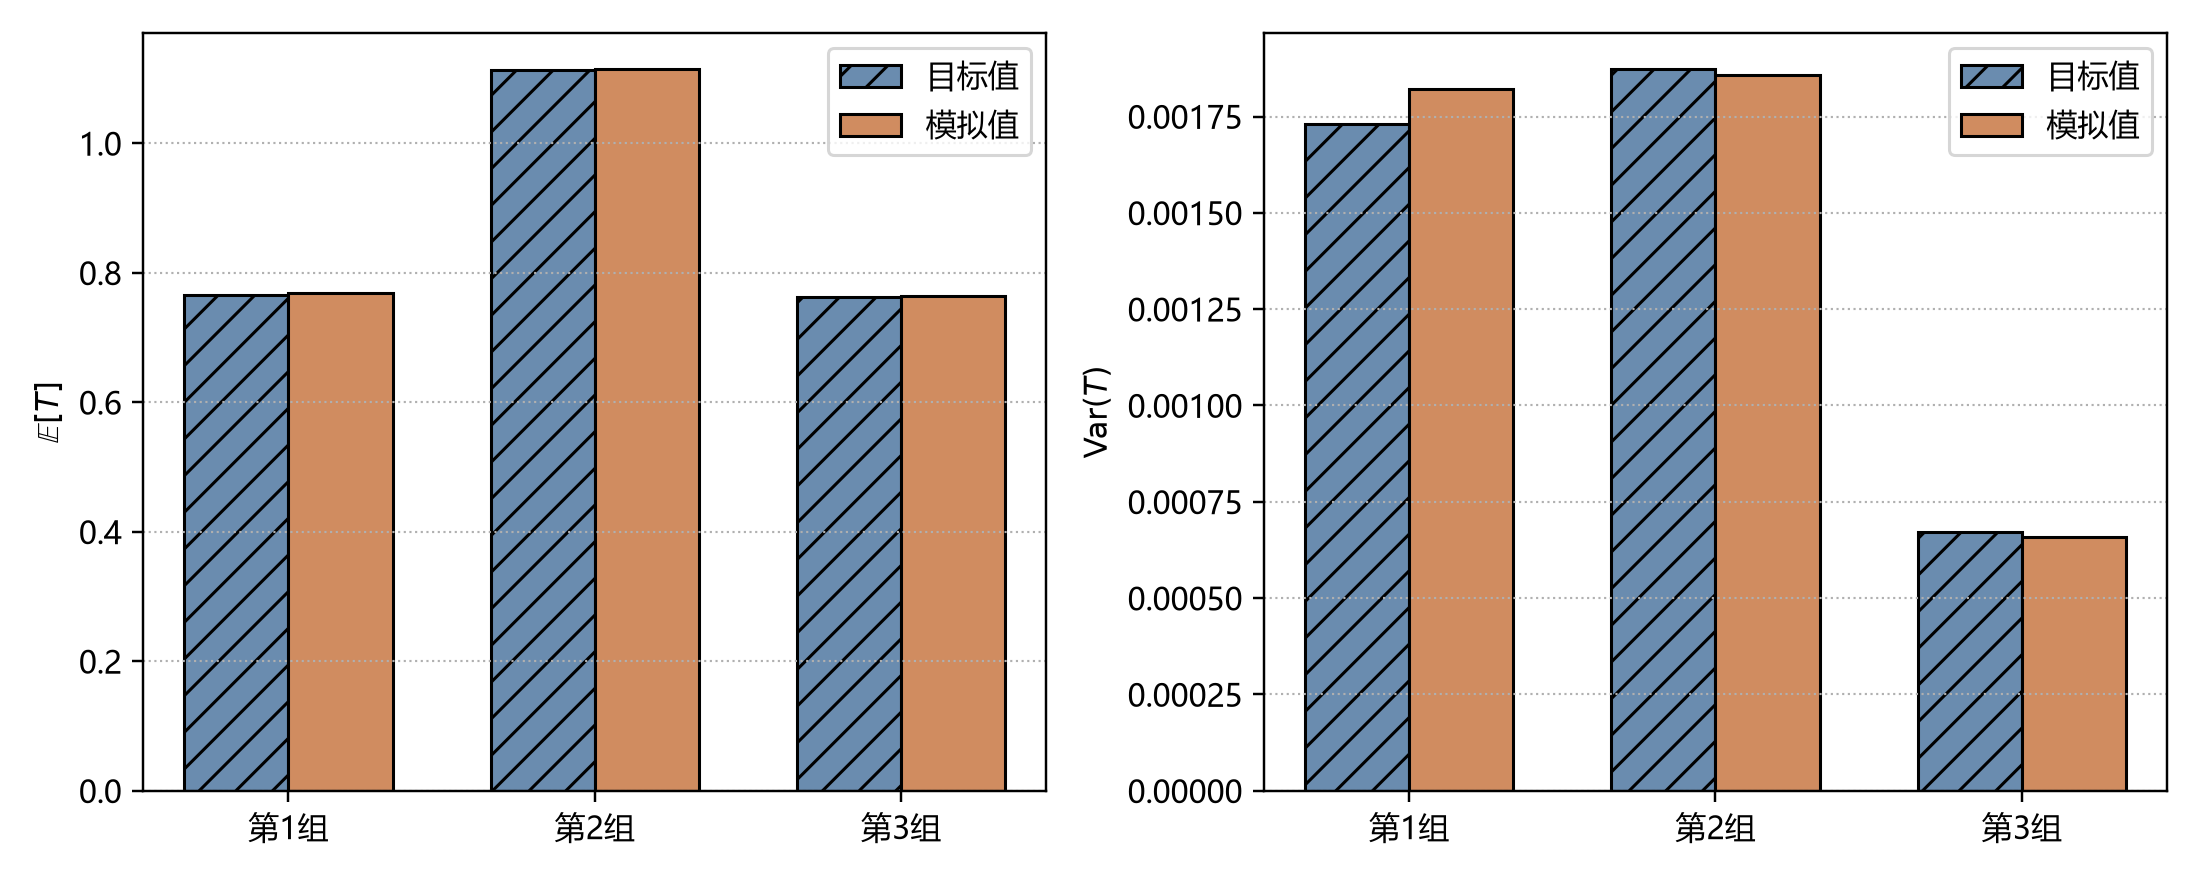
\includegraphics[width=0.88\textwidth]{python/Q1_outputs/target_vs_simulated.png}
\caption{第1题第2小问目标矩与模拟矩对比}
\label{fig:q1_target_vs_simulated}
\end{figure}

图~\ref{fig:q1_target_vs_simulated} 比较了三组随机参数下的目标值和模拟值. 左图为 \(\mathbb E[T]\),  右图为 \(\operatorname{Var}(T)\). 可以看到,  三组实验中模拟均值均与目标均值非常接近,  模拟方差也与目标方差基本一致. 这说明由小噪声展开得到的参数构造能够有效控制脉冲间隔的前两阶矩.

\begin{figure}[htbp]
\centering
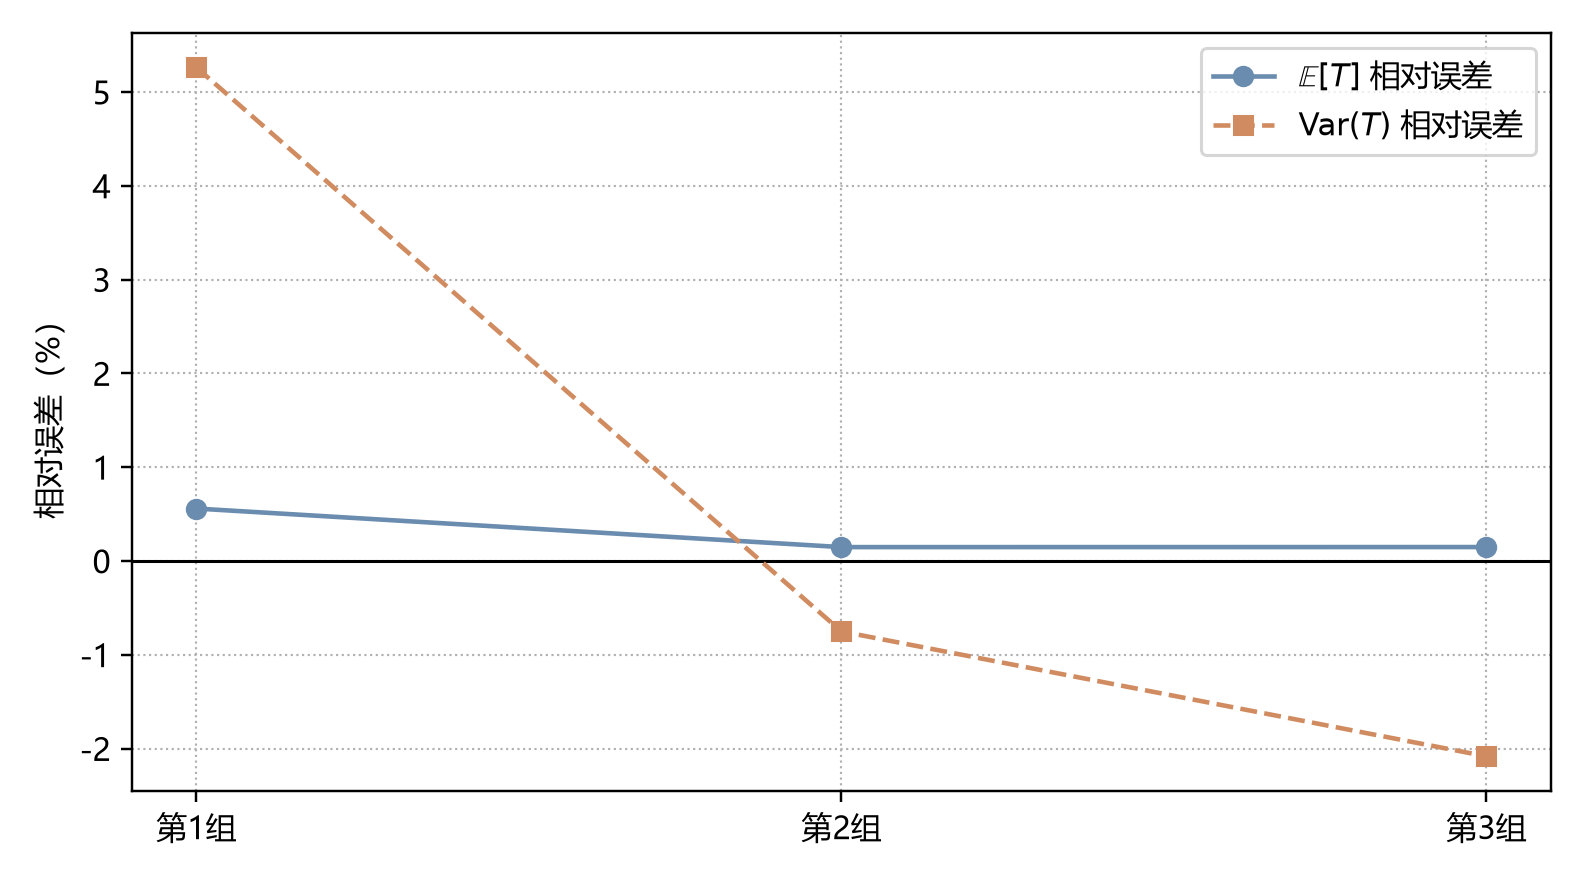
\includegraphics[width=0.78\textwidth]{python/Q1_outputs/relative_errors.png}
\caption{第1题第2小问目标矩与模拟矩的相对误差}
\label{fig:q1_relative_errors}
\end{figure}

图~\ref{fig:q1_relative_errors} 进一步给出了相对误差. 本次数值实验中,  三组实验的均值相对误差均低于 \(1\%\),  方差相对误差也保持在较小范围内. 由于理论推导中使用的是小噪声展开,  方差项对噪声强度更敏感,  因此方差误差通常会比均值误差略大. 但整体误差较小,  说明在所选随机参数范围内,  该近似构造是有效的.

\begin{figure}[htbp]
\centering
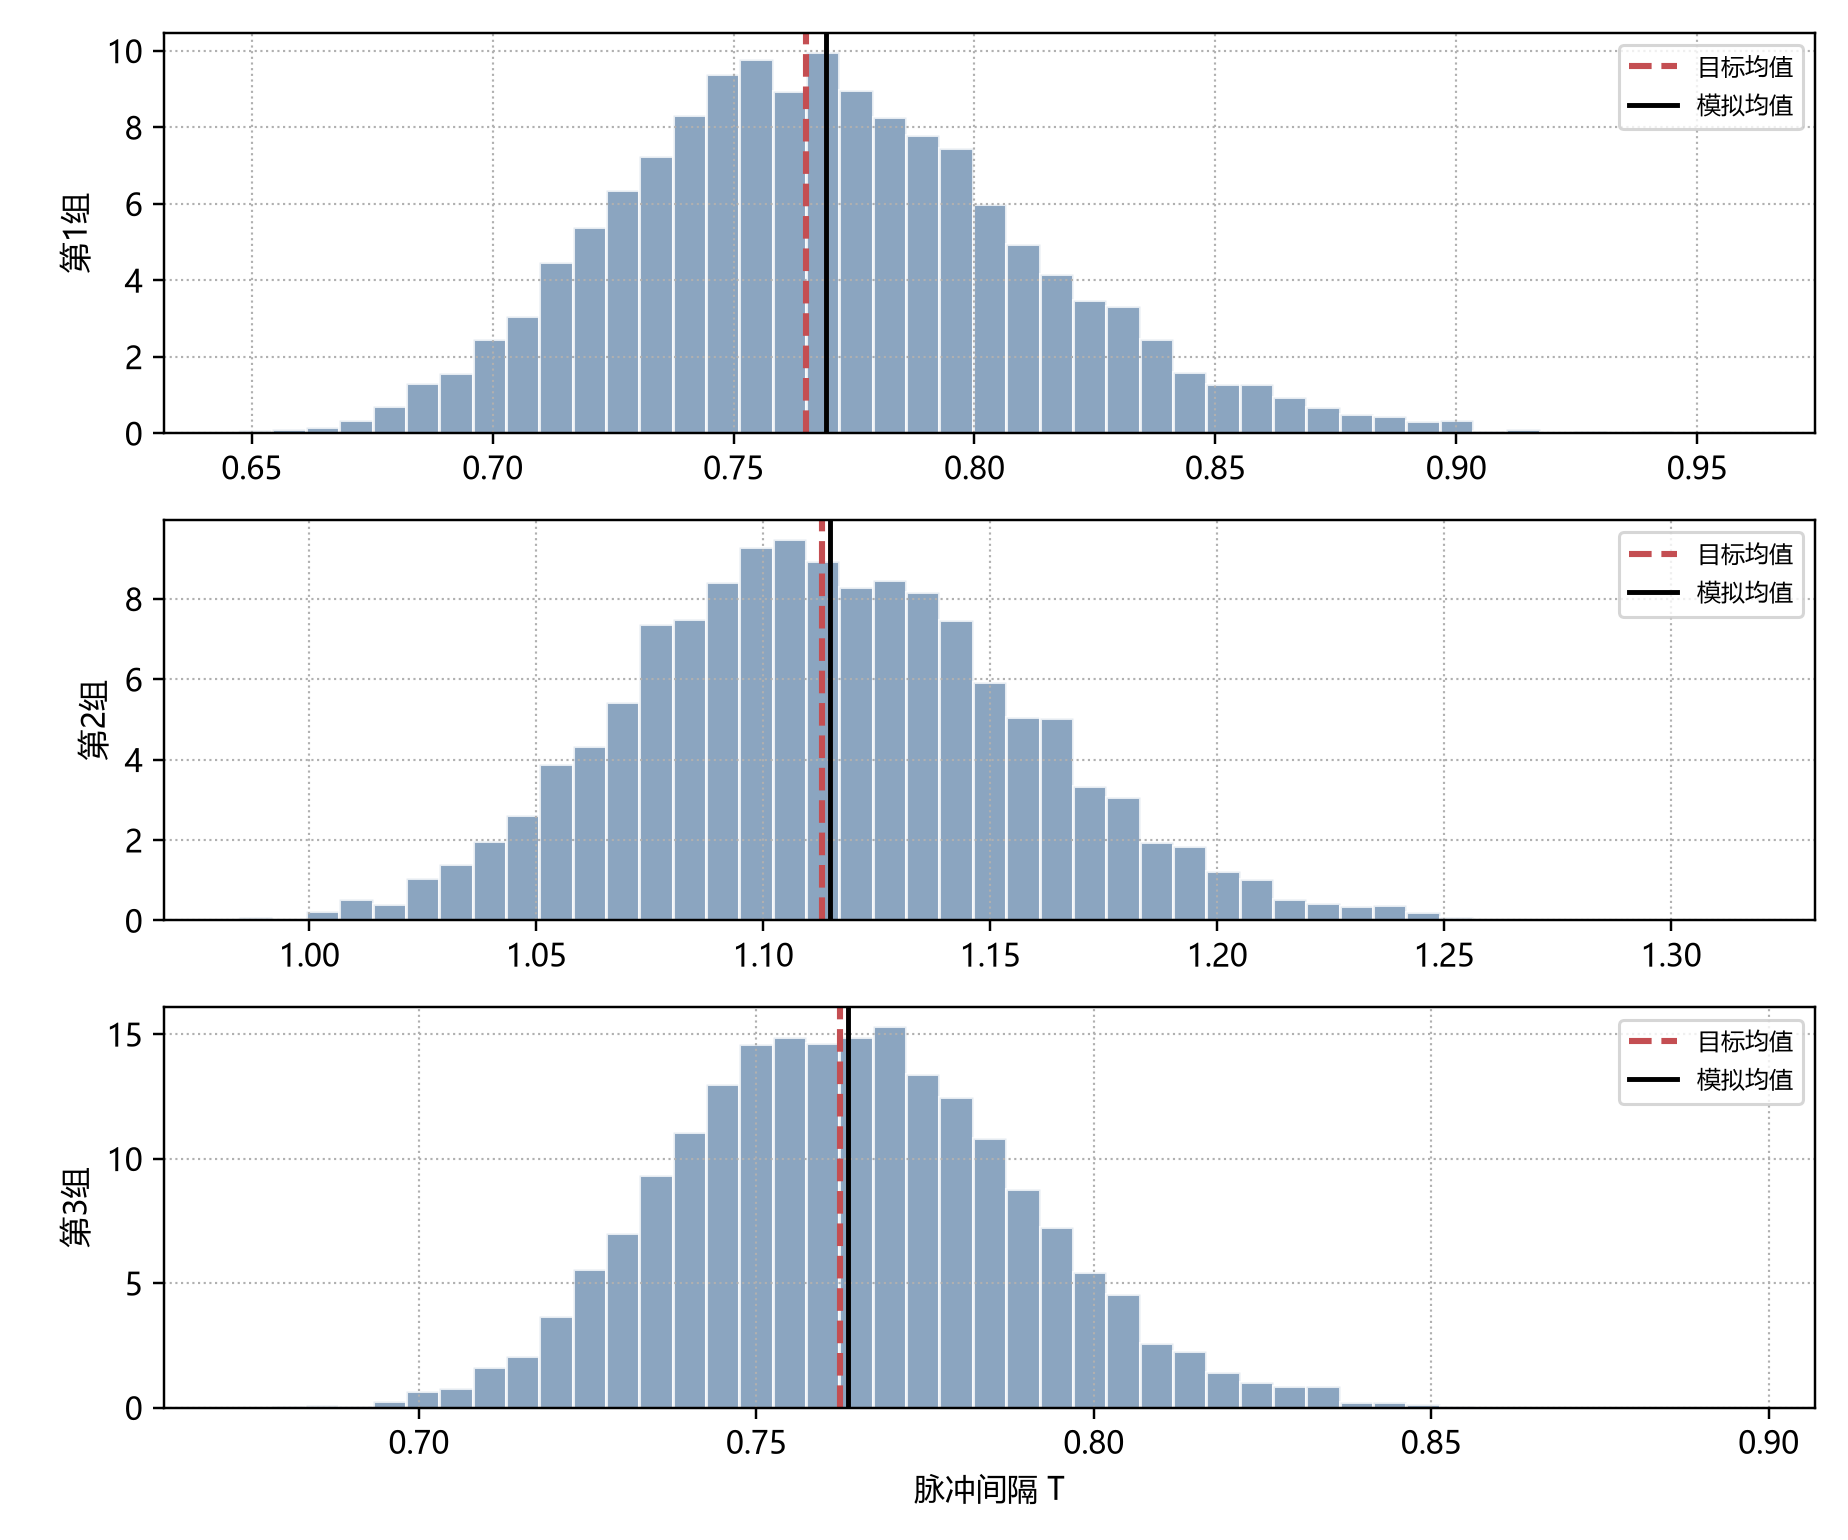
\includegraphics[width=0.88\textwidth]{python/Q1_outputs/interval_histograms.png}
\caption{第1题第2小问三组实验的脉冲间隔分布}
\label{fig:q1_interval_histograms}
\end{figure}

图~\ref{fig:q1_interval_histograms} 展示了三组 Monte Carlo 模拟得到的脉冲间隔 \(T\) 的经验分布. 红色虚线表示目标均值 \(m\),  黑色实线表示模拟均值. 三组实验中两条竖线基本重合,  再次说明构造出的参数能够使 \(\mathbb E[T]\) 接近预设目标. 同时,  直方图的宽度与前面方差图中的结果相对应,  反映了通过 \(\beta=g_{\mathrm{syn}}\sigma_I\) 调节噪声强度可以控制 \(T\) 的波动大小.

\iffalse
\section{第2题}
\subsection{问题重述与记号约定}

考虑一个 ordinary renewal process.设相邻动作电位之间的时间间隔为
$
X_i(i=1,  2, \ldots)$, 
并假设它们独立同分布且$m$阶矩已知(原题的``各阶统计量"在此处理解为$m$阶矩).
记
$S_k=X_1+X_2+\cdots+X_k (k=1,  2,  \ldots),  
$
并约定
$
S_0=0.$
定义到时刻 $t$ 的动作电位发放次数为
$
N(t)=\max\{k: S_k\leq t\}, 
$
其更新函数为
$
M(t)=\mathbb{E}[N(t)].
$
现在要求解$M(t)$的$m$阶矩的表达式.

\textbf{注:}由于$M(t)$是随机变量$N(t)$的期望,  因此$M(t)$是确定的函数了. 笔者猜测可能是题目描述有笔误,  下面分别求解$M(t)$的表达式, $N(t)$的$m$阶矩.

\textbf{注:}另一个问题: $M(t)$的表达式, $N(t)$的$m$阶矩不能仅用$X_i$的m阶矩表示出来,  需要用到$X_i$的完整分布,  但是这是未知的.
\subsection{求解}
设$X_n$的分布函数为
$
F(t)=P(X_i\leq t),  
$
其密度记为
$
f(t)=F'(t).
$
由于 $X_1,  X_2,  \ldots$ 独立同分布,  $S_k$ 的分布函数为 $F$ 的 $k$ 重卷积:
\[
P(S_k\leq t)=F^{*k}(t).
\]
若 $X_i$ 有密度 $f$,  则
\[
f_{S_k}(t)=f^{*k}(t),  
\]
其中
\[
f^{*1}(t)=f(t),  
\]
\[
f^{*2}(t)=\int_0^t f(x)f(t-x)\,  dx,  
\]
一般地,  
\[
f^{*k}(t)
=
\int_0^t f^{*(k-1)}(t-x)f(x)\,  dx.
\]


由于事件 $\{S_k\leq t\}$ 表示第 $k$ 次动作电位已经在 $t$ 之前发生,  因此
\[
N(t)=\sum_{k=1}^{\infty}\mathbf 1_{\{S_k\leq t\}}.
\]
故
\[
M(t)
=\mathbb{E}[N(t)]
=\mathbb{E}\left[
\sum_{k=1}^{\infty}\mathbf 1_{\{S_k\leq t\}}
\right]
=\sum_{k=1}^{\infty}
\mathbb{E}\left[
\mathbf 1_{\{S_k\leq t\}}
\right]
=\sum_{k=1}^{\infty}
P(S_k\leq t)
=
\sum_{k=1}^{\infty}F^{*k}(t).
\]
这就是 ordinary renewal process 的更新函数.若把初始时刻 $S_0=0$ 也计入更新,  则可定义
\[
U(t)=1+M(t)=\sum_{k=0}^{\infty}F^{*k}(t),  
\]
其中 $F^{*0}$ 表示在 $0$ 点的单位质量.

若 $F$ 存在密度 $f$,  则更新函数 $M(t)$ 的导数称为更新密度,  记为
\[
u(t)=M'(t).
\]
由
\[
M(t)=\sum_{k=1}^{\infty}F^{*k}(t)
\]
两边对 $t$ 求导,  得到
\[
u(t)=\sum_{k=1}^{\infty}f^{*k}(t)
.
\]
这个式子说明:$u(t)$ 是时刻 $t$ 出现一次动作电位的总概率密度,  它包含了从初始时刻到 $t$ 之间可能发生任意次数中间放电的情形.

由卷积结构可得
\[
u(t)
=
f(t)+\int_0^t u(t-s)f(s)\,  ds,  
\]
即
\[
u=f+u*f
.
\]
记更新间隔 $X$ 的 Laplace 变换为
\[
\phi(s)=E[e^{-sX}]
=
\int_0^\infty e^{-st}f(t)\,  dt.
\]
对
\[
u(t)=\sum_{k=1}^{\infty}f^{*k}(t)
\]
作 Laplace 变换,  利用卷积在 Laplace 变换下变为乘积,  得
\[
\widehat u(s)
=
\sum_{k=1}^{\infty}\phi(s)^k.
\]
当 $|\phi(s)|<1$ 时,  
\[
\widehat u(s)
=
\frac{\phi(s)}{1-\phi(s)}.
\]
因此
\[
\widehat u(s)=\frac{\phi(s)}{1-\phi(s)}
.
\]
又因为
\[
M(t)=\int_0^t u(x)\,  dx,  
\]
所以
\[
\widehat M(s)
=
\frac{1}{s}\frac{\phi(s)}{1-\phi(s)}
.
\]

接下来推导动作电位发放的 $n$ 阶统计量.将动作电位序列表示为点过程
\[
Y(t)=\sum_{k=1}^{\infty}\delta(t-S_k).
\]
其 $n$ 阶联合强度或 $n$ 阶统计量定义为
\[
G_n(t_1,  \ldots,  t_n)
=
E\left[
Y(t_1)Y(t_2)\cdots Y(t_n)
\right],  
\]
即当 $t_1,  \ldots,  t_n$ 互不相同时,  
\[
P\{\text{在每个 }[t_i,  t_i+dt_i]\text{ 中都有一次放电}\}
\approx
G_n(t_1,  \ldots,  t_n)\,  dt_1\cdots dt_n.
\]

先考虑
\[
0<t_1<t_2<\cdots<t_n.
\]
令
\[
t_0=0,  
\]
并定义相邻指定发放时刻之间的时间差为
\[
\Delta_j=t_j-t_{j-1},  \qquad j=1,  2,  \ldots,  n.
\]
也就是说,  
\[
\Delta_1=t_1,  \qquad
\Delta_2=t_2-t_1,  \qquad \ldots,  \qquad
\Delta_n=t_n-t_{n-1}.
\]

从 $0$ 到 $t_1$ 之间,  可能经过 $k_1$ 个更新间隔后在 $t_1$ 发生放电,  其密度为
\[
f^{*k_1}(\Delta_1).
\]
从 $t_1$ 到 $t_2$ 之间,  可能经过 $k_2$ 个更新间隔后在 $t_2$ 发生放电,  其密度为
\[
f^{*k_2}(\Delta_2).
\]
一般地,  从 $t_{j-1}$ 到 $t_j$ 之间,  可能经过 $k_j$ 个更新间隔后在 $t_j$ 发生放电,  其密度为
\[
f^{*k_j}(\Delta_j).
\]
这里
\[
k_j=1,  2,  \ldots
\]
因为两个指定的放电时刻之间至少要跨过一个更新间隔;若 $k_j>1$,  则说明两个指定放电时刻之间还存在未被指定的中间放电.

由于 ordinary renewal process 在每次放电后重新开始,  且之后的更新间隔与过去独立,  因此在给定
\[
k_1,  k_2,  \ldots,  k_n
\]
的条件下,  联合密度为
\[
f^{*k_1}(\Delta_1)
f^{*k_2}(\Delta_2)
\cdots
f^{*k_n}(\Delta_n).
\]
对所有可能的 $k_1,  \ldots,  k_n$ 求和,  得到
\[
G_n(t_1,  \ldots,  t_n)
=
\sum_{k_1=1}^{\infty}
\cdots
\sum_{k_n=1}^{\infty}
\prod_{j=1}^{n}f^{*k_j}(\Delta_j).
\]
由于各个求和变量彼此独立,  上式可写为
\[
G_n(t_1,  \ldots,  t_n)
=
\prod_{j=1}^{n}
\left[
\sum_{k_j=1}^{\infty}f^{*k_j}(\Delta_j)
\right].
\]
根据更新密度的定义
\[
u(t)=\sum_{k=1}^{\infty}f^{*k}(t),  
\]
于是
\[
G_n(t_1,  \ldots,  t_n)
=
\prod_{j=1}^{n}u(\Delta_j)
.
\]
即
\[
G_n(t_1,  \ldots,  t_n)
=
u(t_1)u(t_2-t_1)\cdots u(t_n-t_{n-1})
,  
\qquad
0<t_1<t_2<\cdots<t_n.
\]

若 $t_1,  \ldots,  t_n$ 未按时间顺序排列,  设其升序排列为
\[
t_{(1)}<t_{(2)}<\cdots<t_{(n)},  
\]
并令
\[
t_{(0)}=0.
\]
则有
\[
G_n(t_1,  \ldots,  t_n)
=
\prod_{j=1}^{n}
u\left(t_{(j)}-t_{(j-1)}\right)
.
\]
等价地,  可以写成对所有排列求和的形式:
\[
G_n(t_1,  \ldots,  t_n)
=
\sum_{\pi\in S_n}
\mathbf 1_{\{0<t_{\pi(1)}<\cdots<t_{\pi(n)}\}}
\prod_{j=1}^{n}
u\left(t_{\pi(j)}-t_{\pi(j-1)}\right)
,  
\]
其中
\[
t_{\pi(0)}=0.
\]
在这个表达式中,  实际上只有使时间升序排列的那个排列会贡献非零项.

如果已知更新间隔 $X$ 的各阶矩
\[
\mu_r=E[X^r],  
\qquad r=1,  2,  \ldots,  
\]
并且这些矩能够唯一确定 $X$ 的分布,  则
\[
\phi(s)=E[e^{-sX}]
=
\sum_{r=0}^{\infty}\frac{(-s)^r}{r!}\mu_r,  
\]
其中
\[
\mu_0=1.
\]
若已知的是累积量 $\kappa_r$,  则
\[
\phi(s)
=
\exp\left(
\sum_{r=1}^{\infty}
\frac{(-s)^r}{r!}\kappa_r
\right).
\]
由
\[
\widehat u(s)=\frac{\phi(s)}{1-\phi(s)}
\]
即可得到 $u(t)$.因此,  在
\[
0<t_1<t_2<\cdots<t_n
\]
时,  令
\[
\Delta_j=t_j-t_{j-1},  
\qquad t_0=0,  
\]
则动作电位发放的 $n$ 阶统计量可写为
\[
G_n(t_1,  \ldots,  t_n)
=
\prod_{j=1}^{n}u(\Delta_j)
.
\]
其关于 $\Delta_1,  \ldots,  \Delta_n$ 的多维 Laplace 变换为
\[
\widehat G_n(s_1,  \ldots,  s_n)
=
\prod_{j=1}^{n}
\frac{\phi(s_j)}{1-\phi(s_j)}
.
\]
等价地,  
\[
G_n(t_1,  \ldots,  t_n)
=
\mathcal L^{-1}_{s_1,  \ldots,  s_n}
\left[
\prod_{j=1}^{n}
\frac{\phi(s_j)}{1-\phi(s_j)}
\right]
(\Delta_1,  \ldots,  \Delta_n)
.
\]

特别地,  一阶统计量为
\[
G_1(t)=u(t).
\]
二阶统计量为
\[
G_2(t_1,  t_2)
=
u(t_1)u(t_2-t_1),  
\qquad 0<t_1<t_2.
\]
三阶统计量为
\[
G_3(t_1,  t_2,  t_3)
=
u(t_1)u(t_2-t_1)u(t_3-t_2),  
\qquad 0<t_1<t_2<t_3.
\]
一般地,  
\[
G_n(t_1,  \ldots,  t_n)
=
u(t_1)u(t_2-t_1)\cdots u(t_n-t_{n-1})
.
\]

如果题目中的 ``$n$ 阶统计量'' 指的是计数过程 $N(t)$ 的 $n$ 阶矩,  则可进一步得到如下表达式.定义下降阶乘矩
\[
(N(t))_r
=
N(t)(N(t)-1)\cdots(N(t)-r+1).
\]
可以证明
\[
E[(N(t))_r]
=
r!
\sum_{k=r}^{\infty}
\binom{k-1}{r-1}
F^{*k}(t)
.
\]
理由如下:$(N(t))_r$ 表示从 $N(t)$ 个放电时刻中选出有顺序的 $r$ 个放电时刻的数量.若这些放电时刻中最大的指标为 $k$,  则相应事件等价于
\[
S_k\leq t.
\]
在固定最大指标为 $k$ 时,  需要从 $1,  \ldots,  k-1$ 中再选出 $r-1$ 个指标,  共有
\[
\binom{k-1}{r-1}
\]
种选法;由于是有顺序的 $r$ 元组,  还需乘以 $r!$.因此
\[
E[(N(t))_r]
=
r!
\sum_{k=r}^{\infty}
\binom{k-1}{r-1}
P(S_k\leq t),  
\]
即
\[
E[(N(t))_r]
=
r!
\sum_{k=r}^{\infty}
\binom{k-1}{r-1}
F^{*k}(t).
\]
普通矩与下降阶乘矩之间满足
\[
N(t)^n
=
\sum_{r=1}^{n}
\left\{ {n\atop r} \right\}
(N(t))_r,  
\]
其中
\[
\left\{ {n\atop r} \right\}
\]
表示第二类 Stirling 数.因此
\[
E[N(t)^n]
=
\sum_{r=1}^{n}
\left\{ {n\atop r} \right\}
r!
\sum_{k=r}^{\infty}
\binom{k-1}{r-1}
F^{*k}(t)
.
\]
当 $n=1$ 时,  上式退化为
\[
E[N(t)]
=
\sum_{k=1}^{\infty}F^{*k}(t)
=
M(t),  
\]
正好得到更新函数.

\textcolor{red}{另一个答案}

\paragraph{解.}
设更新间隔 \(X_1,  X_2, \ldots\) 独立同分布,  其分布函数记为
\[
    F(t)=\mathbb P(X_1\leq t).
\]
令
\[
    S_k=X_1+X_2+\cdots+X_k, \qquad k=1,  2, \ldots, 
\]
并约定 \(S_0=0\). 到时刻 \(t\) 为止的动作电位发放次数为
\[
    N(t)=\max\{k: S_k\leq t\}.
\]
由于事件 \(\{N(t)\geq k\}\) 等价于事件 \(\{S_k\leq t\}\),  因此有
\[
    \mathbb P(N(t)\geq k)
    =
    \mathbb P(S_k\leq t).
\]
又因为 \(S_k\) 是 \(k\) 个独立同分布更新间隔之和,  所以 \(S_k\) 的分布函数为
\(F\) 的 \(k\) 重卷积,  记为 \(F^{*k}\). 于是
\[
    \mathbb P(S_k\leq t)=F^{*k}(t).
\]

首先,  更新函数定义为
\[
    M(t)=\mathbb E[N(t)].
\]
因为 \(N(t)\) 是非负整数值随机变量,  所以
\[
    \mathbb E[N(t)]
    =
    \sum_{k=1}^{\infty}\mathbb P(N(t)\geq k).
\]
代入上式可得
\[
    M(t)
    =
    \sum_{k=1}^{\infty}F^{*k}(t).
\]
这就是 ordinary renewal process 的更新函数表达式. 它也可写成更新方程
\[
    M(t)=F(t)+\int_0^t M(t-x)\, \mathrm dF(x).
\]

需要注意的是,  \(M(t)=\mathbb E[N(t)]\) 已经是随机变量 \(N(t)\) 的期望, 
因此 \(M(t)\) 本身是关于 \(t\) 的确定性函数,  不是随机变量.
所以严格来说,  \(M(t)\) 没有所谓的 ``\(m\) 阶矩''. 若原题中的
``更新函数的 \(m\) 阶统计量'' 是指发放次数 \(N(t)\) 的 \(m\) 阶矩,  则应求
\[
    \mathbb E[N(t)^m].
\]

对任意非负整数值随机变量 \(Y\),  有恒等式
\[
    Y^m
    =
    \sum_{k=1}^{Y}\left(k^m-(k-1)^m\right).
\]
令 \(Y=N(t)\),  两边取期望,  得
\[
    \mathbb E[N(t)^m]
    =
    \sum_{k=1}^{\infty}
    \left(k^m-(k-1)^m\right)
    \mathbb P(N(t)\geq k).
\]
再利用
\[
    \mathbb P(N(t)\geq k)=F^{*k}(t), 
\]
得到
\[
    \boxed{
    \mathbb E[N(t)^m]
    =
    \sum_{k=1}^{\infty}
    \left(k^m-(k-1)^m\right)F^{*k}(t)
    }.
\]

特别地,  当 \(m=1\) 时, 
\[
    \mathbb E[N(t)]
    =
    \sum_{k=1}^{\infty}F^{*k}(t)
    =
    M(t), 
\]
这与更新函数的定义一致.

因此,  若严格按照更新函数的定义,  应有
\[
    \boxed{
    M(t)=\sum_{k=1}^{\infty}F^{*k}(t)
    }.
\]
若将题目中的 ``更新函数的 \(m\) 阶统计量'' 理解为发放次数 \(N(t)\) 的
\(m\) 阶矩,  则有
\[
    \boxed{
    \mathbb E[N(t)^m]
    =
    \sum_{k=1}^{\infty}
    \left(k^m-(k-1)^m\right)F^{*k}(t)
    }.
\]

此外,  仅知道更新间隔 \(X_i\) 的有限阶矩通常不足以唯一确定
\(M(t)\) 或 \(\mathbb E[N(t)^m]\). 上述表达式实际依赖于 \(X_i\) 的分布函数
\(F\),  或等价地依赖于 \(S_k\) 的分布 \(F^{*k}\).
\fi

\iffalse
\section{第3题}

考虑如下兴奋--抑制神经网络模型:
\[
\tau_E\frac{dv_E}{dt}
=
-v_E+\left[M_{EE}v_E-M_{EI}v_I+h_E\right]^+,  
\]
\[
\tau_I\frac{dv_I}{dt}
=
-v_I+\left[M_{IE}v_E-M_{II}v_I+h_I\right]^+,  
\]
其中
\[
[z]^+=\max\{z,  0\}.
\]
变量 \(v_E\) 和 \(v_I\) 分别表示兴奋性神经元群和抑制性神经元群的放电率;
\(M_{ab}\) 表示对应连接权重,  \(a,  b=E,  I\);
\(h_E,  h_I\) 分别表示兴奋性和抑制性神经元群接收到的外部刺激;
\(\tau_E,  \tau_I>0\) 是时间尺度参数.

为方便书写,  记
\[
u_E=M_{EE}v_E-M_{EI}v_I+h_E,  
\]
\[
u_I=M_{IE}v_E-M_{II}v_I+h_I.
\]
则系统可写为
\[
\tau_E\dot v_E=-v_E+[u_E]^+,  
\]
\[
\tau_I\dot v_I=-v_I+[u_I]^+.
\]

由于函数 \([z]^+=\max\{z,  0\}\) 在 \(z=0\) 处不可导,  因此经典 Hopf 分叉只能在平衡点满足
\[
u_E^*>0,  \qquad u_I^*>0
\]
的光滑区域中讨论.若平衡点位于 \(u_E=0\) 或 \(u_I=0\) 的阈值边界上,  则对应的是非光滑分叉,  而不是经典意义下的 Hopf 分叉.

\subsection{平衡点与分区讨论}

在平衡点 \((v_E^*,  v_I^*)\) 处,  有
\[
v_E^*=[u_E^*]^+,  
\]
\[
v_I^*=[u_I^*]^+.
\]
因此必有
\[
v_E^*\ge 0,  \qquad v_I^*\ge 0.
\]

令
\[
\sigma_E=
\begin{cases}
1,   & u_E>0,  \\
0,   & u_E<0,  
\end{cases}
\qquad
\sigma_I=
\begin{cases}
1,   & u_I>0,  \\
0,   & u_I<0.
\end{cases}
\]
在某个光滑分区内,  系统的 Jacobian 矩阵为
\[
J_{\sigma_E,  \sigma_I}
=
\begin{pmatrix}
\dfrac{-1+\sigma_E M_{EE}}{\tau_E}
&
-\dfrac{\sigma_E M_{EI}}{\tau_E}
\\[1.2em]
\dfrac{\sigma_I M_{IE}}{\tau_I}
&
\dfrac{-1-\sigma_I M_{II}}{\tau_I}
\end{pmatrix}.
\]

若 \(\sigma_E=0,  \sigma_I=0\),  则
\[
J_{0,  0}
=
\begin{pmatrix}
-\dfrac1{\tau_E} & 0\\
0 & -\dfrac1{\tau_I}
\end{pmatrix},  
\]
其两个特征值均为负实数,  因此不可能发生 Hopf 分叉.

若 \(\sigma_E=1,  \sigma_I=0\),  则
\[
J_{1,  0}
=
\begin{pmatrix}
\dfrac{M_{EE}-1}{\tau_E} & -\dfrac{M_{EI}}{\tau_E}\\
0 & -\dfrac1{\tau_I}
\end{pmatrix}.
\]
这是上三角矩阵,  其特征值为
\[
\lambda_1=\frac{M_{EE}-1}{\tau_E},  
\qquad
\lambda_2=-\frac1{\tau_I}.
\]
两个特征值均为实数,  因此也不可能发生 Hopf 分叉.

若 \(\sigma_E=0,  \sigma_I=1\),  则
\[
J_{0,  1}
=
\begin{pmatrix}
-\dfrac1{\tau_E} & 0\\
\dfrac{M_{IE}}{\tau_I} & -\dfrac{1+M_{II}}{\tau_I}
\end{pmatrix}.
\]
这是下三角矩阵,  其特征值为
\[
\lambda_1=-\frac1{\tau_E},  
\qquad
\lambda_2=-\frac{1+M_{II}}{\tau_I}.
\]
两个特征值仍为实数,  因此也不可能发生 Hopf 分叉.

所以,  经典 Hopf 分叉只可能发生在双激活区:
\[
u_E^*>0,  \qquad u_I^*>0.
\]

\subsection{双激活区中的平衡点}

在双激活区中,  
\[
[u_E]^+=u_E,  \qquad [u_I]^+=u_I.
\]
因此系统变为
\[
\tau_E\dot v_E
=
-v_E+M_{EE}v_E-M_{EI}v_I+h_E,  
\]
\[
\tau_I\dot v_I
=
-v_I+M_{IE}v_E-M_{II}v_I+h_I.
\]

令 \(\dot v_E=\dot v_I=0\),  得到平衡方程
\[
0
=
-v_E+M_{EE}v_E-M_{EI}v_I+h_E,  
\]
\[
0
=
-v_I+M_{IE}v_E-M_{II}v_I+h_I.
\]
整理得
\[
(1-M_{EE})v_E+M_{EI}v_I=h_E,  
\]
\[
-M_{IE}v_E+(1+M_{II})v_I=h_I.
\]
写成矩阵形式为
\[
\begin{pmatrix}
1-M_{EE} & M_{EI}\\
-M_{IE} & 1+M_{II}
\end{pmatrix}
\begin{pmatrix}
v_E\\
v_I
\end{pmatrix}
=
\begin{pmatrix}
h_E\\
h_I
\end{pmatrix}.
\]

记
\[
\mathcal D
=
(1-M_{EE})(1+M_{II})+M_{EI}M_{IE}.
\]
若
\[
\mathcal D\ne 0,  
\]
则由二阶线性方程组求解可得
\[
v_E^*
=
\frac{(1+M_{II})h_E-M_{EI}h_I}{\mathcal D},  
\]
\[
v_I^*
=
\frac{M_{IE}h_E+(1-M_{EE})h_I}{\mathcal D}.
\]

由于当前讨论的是双激活区,  因此还必须要求
\[
v_E^*>0,  \qquad v_I^*>0.
\]
在双激活平衡点处有
\[
u_E^*=v_E^*,  \qquad u_I^*=v_I^*,  
\]
所以双激活条件等价于
\[
v_E^*>0,  \qquad v_I^*>0.
\]

\subsection{双激活区的线性化}

在双激活区,  系统为线性仿射系统:
\[
\dot v_E
=
\frac{M_{EE}-1}{\tau_E}v_E
-
\frac{M_{EI}}{\tau_E}v_I
+
\frac{h_E}{\tau_E},  
\]
\[
\dot v_I
=
\frac{M_{IE}}{\tau_I}v_E
-
\frac{1+M_{II}}{\tau_I}v_I
+
\frac{h_I}{\tau_I}.
\]
因此 Jacobian 矩阵为
\[
J
=
\begin{pmatrix}
\dfrac{M_{EE}-1}{\tau_E}
&
-\dfrac{M_{EI}}{\tau_E}
\\[1.2em]
\dfrac{M_{IE}}{\tau_I}
&
-\dfrac{1+M_{II}}{\tau_I}
\end{pmatrix}.
\]

其迹为
\[
T=\operatorname{tr}(J)
=
\frac{M_{EE}-1}{\tau_E}
-
\frac{1+M_{II}}{\tau_I}.
\]

其行列式为
\[
\Delta=\det(J).
\]
直接计算得
\[
\Delta
=
\frac{M_{EE}-1}{\tau_E}
\left(
-\frac{1+M_{II}}{\tau_I}
\right)
-
\left(
-\frac{M_{EI}}{\tau_E}
\right)
\left(
\frac{M_{IE}}{\tau_I}
\right).
\]
即
\[
\Delta
=
\frac{-(M_{EE}-1)(1+M_{II})+M_{EI}M_{IE}}
{\tau_E\tau_I}.
\]
由于
\[
-(M_{EE}-1)(1+M_{II})
=
(1-M_{EE})(1+M_{II}),  
\]
所以
\[
\Delta
=
\frac{(1-M_{EE})(1+M_{II})+M_{EI}M_{IE}}
{\tau_E\tau_I}.
\]
因此
\[
\Delta=\frac{\mathcal D}{\tau_E\tau_I}.
\]

Jacobian 的特征方程为
\[
\lambda^2-T\lambda+\Delta=0.
\]
在二维系统中,  经典 Hopf 分叉的线性条件为
\[
T=0,  \qquad \Delta>0.
\]

\subsection{以 \(\tau_I\) 为分叉参数的 Hopf 条件}

现在固定其余参数,  只令 \(\tau_I\) 变化.

由 Hopf 条件的第一条
\[
T=0,  
\]
可得
\[
\frac{M_{EE}-1}{\tau_E}
-
\frac{1+M_{II}}{\tau_I}
=0.
\]
因此
\[
\frac{M_{EE}-1}{\tau_E}
=
\frac{1+M_{II}}{\tau_I}.
\]
解得临界值
\[
\tau_I^H
=
\frac{\tau_E(1+M_{II})}{M_{EE}-1}.
\]

为了使
\[
\tau_I^H>0,  
\]
在通常假设
\[
M_{II}>0
\]
的情况下,  需要
\[
M_{EE}>1.
\]

Hopf 条件的第二条为
\[
\Delta>0.
\]
由于
\[
\Delta=\frac{\mathcal D}{\tau_E\tau_I},  
\]
且
\[
\tau_E>0,  \qquad \tau_I>0,  
\]
所以
\[
\Delta>0
\iff
\mathcal D>0.
\]
即
\[
(1-M_{EE})(1+M_{II})+M_{EI}M_{IE}>0.
\]

当 \(M_{EE}>1\) 时,  上式等价于
\[
M_{EI}M_{IE}>(M_{EE}-1)(1+M_{II}).
\]

因此,  以 \(\tau_I\) 为分叉参数时,  Hopf 分叉的临界条件为
\[
\tau_I^H
=
\frac{\tau_E(1+M_{II})}{M_{EE}-1}
\]
并且需要满足
\[
M_{EE}>1,  
\qquad
M_{EI}M_{IE}>(M_{EE}-1)(1+M_{II}).
\]
同时,  平衡点必须位于双激活区,  即
\[
v_E^*>0,  \qquad v_I^*>0.
\]

\subsection{Hopf 分叉处的频率}

在 Hopf 点处,  
\[
T=0.
\]
因此特征方程变为
\[
\lambda^2+\Delta=0.
\]
于是
\[
\lambda=\pm i\sqrt{\Delta}.
\]
Hopf 分叉处的角频率为
\[
\omega_H=\sqrt{\Delta_H}.
\]

由于
\[
\Delta_H
=
\frac{\mathcal D}{\tau_E\tau_I^H},  
\]
代入
\[
\tau_I^H
=
\frac{\tau_E(1+M_{II})}{M_{EE}-1},  
\]
得到
\[
\Delta_H
=
\frac{\mathcal D}{\tau_E}
\frac{M_{EE}-1}{\tau_E(1+M_{II})}.
\]
因此
\[
\omega_H
=
\sqrt{
\frac{\mathcal D(M_{EE}-1)}
{\tau_E^2(1+M_{II})}
}.
\]

其中
\[
\mathcal D
=
(1-M_{EE})(1+M_{II})+M_{EI}M_{IE}.
\]

\subsection{横截性条件}

经典 Hopf 分叉还要求特征值实部横截穿过虚轴.

当特征值为一对共轭复根时,  由
\[
\lambda^2-T\lambda+\Delta=0
\]
可知,  特征值实部为
\[
\operatorname{Re}\lambda=\frac{T}{2}.
\]
因此
\[
\frac{d}{d\tau_I}\operatorname{Re}\lambda
=
\frac12\frac{dT}{d\tau_I}.
\]

又因为
\[
T(\tau_I)
=
\frac{M_{EE}-1}{\tau_E}
-
\frac{1+M_{II}}{\tau_I},  
\]
所以
\[
\frac{dT}{d\tau_I}
=
\frac{1+M_{II}}{\tau_I^2}.
\]
于是
\[
\left.
\frac{d}{d\tau_I}\operatorname{Re}\lambda
\right|_{\tau_I=\tau_I^H}
=
\frac{1+M_{II}}{2(\tau_I^H)^2}.
\]
由于
\[
M_{II}>0,  \qquad \tau_I^H>0,  
\]
所以
\[
\left.
\frac{d}{d\tau_I}\operatorname{Re}\lambda
\right|_{\tau_I=\tau_I^H}
>0.
\]
因此横截性条件成立.

进一步,  当
\[
\tau_I<\tau_I^H
\]
时,  
\[
T<0,  
\]
平衡点为稳定焦点;当
\[
\tau_I>\tau_I^H
\]
时,  
\[
T>0,  
\]
平衡点为不稳定焦点.

\subsection{关于退化 Hopf 的说明}

虽然上述线性 Hopf 条件和横截性条件成立,  但是需要注意:在双激活区内,  本模型是严格的线性仿射系统.令
\[
x=v_E-v_E^*,  
\qquad
y=v_I-v_I^*.
\]
则在平衡点附近,  只要轨道仍处于双激活区,  就有
\[
\begin{pmatrix}
\dot x\\
\dot y
\end{pmatrix}
=
J
\begin{pmatrix}
x\\
y
\end{pmatrix}.
\]
因此局部系统没有二次项,  三次项或更高阶非线性项.

普通 Hopf 分叉的正规形通常写为
\[
\dot z=(\alpha+i\omega)z+l_1z|z|^2+\cdots,  
\]
其中 \(l_1\) 为第一 Lyapunov 系数,  用来判断超临界或亚临界 Hopf 分叉.而在本模型的双激活区中,  局部非线性项为零,  因此
\[
l_1=0.
\]
所以这是一个退化 Hopf,  而不是普通非退化 Hopf.

在 \(\tau_I=\tau_I^H\) 时,  双激活区附近表现为线性中心.为了说明这一点,  记
\[
a=\frac{M_{EE}-1}{\tau_E},  
\qquad
p=\frac{M_{EI}}{\tau_E},  
\qquad
q=\frac{M_{IE}}{\tau_I^H}.
\]
则 Hopf 点处的线性矩阵为
\[
J_H=
\begin{pmatrix}
a & -p\\
q & -a
\end{pmatrix}.
\]
此时
\[
pq-a^2>0.
\]
考虑二次型
\[
Q(x,  y)=qx^2-2axy+py^2.
\]
沿着线性系统
\[
\dot x=ax-py,  
\]
\[
\dot y=qx-ay
\]
求导,  得到
\[
\frac{dQ}{dt}
=
2qx\dot x-2a(\dot xy+x\dot y)+2py\dot y.
\]
代入 \(\dot x=ax-py\),  \(\dot y=qx-ay\),  有
\[
\frac{dQ}{dt}
=
2qx(ax-py)
-2a\big((ax-py)y+x(qx-ay)\big)
+2py(qx-ay).
\]
展开得
\[
\frac{dQ}{dt}
=
2aqx^2-2pqxy
-2a(qx^2-py^2)
+2pqxy-2apy^2.
\]
继续整理:
\[
\frac{dQ}{dt}
=
2aqx^2-2pqxy
-2aqx^2+2apy^2
+2pqxy-2apy^2=0.
\]
因此
\[
Q(x,  y)=\text{常数}.
\]
这说明临界点附近是一族闭轨道,  而不是普通 Hopf 分叉中由非线性项产生的唯一小振幅极限环.

当 \(\tau_I>\tau_I^H\) 时,  平衡点附近轨道会向外螺旋.由于 ReLU 阈值会使系统进入其他分段线性区域,  完整系统可能在全局上形成有限振幅周期振荡.但这种振荡来自分段线性系统的全局阈值效应,  而不是普通局部 Hopf 定理直接给出的极限环.

\subsection{以 \(h_E\) 为分叉参数的讨论}

现在固定其他参数,  只改变 \(h_E\).

在双激活区中,  平衡点为
\[
v_E^*
=
\frac{(1+M_{II})h_E-M_{EI}h_I}{\mathcal D},  
\]
\[
v_I^*
=
\frac{M_{IE}h_E+(1-M_{EE})h_I}{\mathcal D}.
\]
因此,  改变 \(h_E\) 会改变平衡点的位置.

但是双激活区中的 Jacobian 矩阵为
\[
J
=
\begin{pmatrix}
\dfrac{M_{EE}-1}{\tau_E}
&
-\dfrac{M_{EI}}{\tau_E}
\\[1.2em]
\dfrac{M_{IE}}{\tau_I}
&
-\dfrac{1+M_{II}}{\tau_I}
\end{pmatrix}.
\]
可以看到,  \(J\) 不含 \(h_E\).因此
\[
T=
\frac{M_{EE}-1}{\tau_E}
-
\frac{1+M_{II}}{\tau_I}
\]
不含 \(h_E\),  并且
\[
\Delta
=
\frac{\mathcal D}{\tau_E\tau_I}
\]
也不含 \(h_E\).

于是
\[
\frac{d}{dh_E}\operatorname{Re}\lambda=0.
\]
这说明
\[
h_E\text{ 不是该 ReLU 模型双激活区中的经典 Hopf 分叉参数.}
\]

具体来说,  若
\[
\tau_I\ne \tau_I^H,  
\]
则改变 \(h_E\) 不会让特征值穿过虚轴,  因此不会发生 Hopf 分叉.

若
\[
\tau_I=\tau_I^H,  
\]
则只要平衡点仍然位于双激活区,  所有满足条件的 \(h_E\) 都对应一对纯虚特征值.但这不是关于 \(h_E\) 的横截穿越,  因为
\[
\frac{d}{dh_E}\operatorname{Re}\lambda=0.
\]
所以这不是非退化 Hopf 分叉.

在 \((\tau_I,  h_E)\) 参数平面中,  经典 Hopf 条件给出的是
\[
\tau_I
=
\frac{\tau_E(1+M_{II})}{M_{EE}-1},  
\]
而 \(h_E\) 的作用只是改变平衡点的位置,  并要求平衡点仍处于双激活区.

当 \(\mathcal D>0\) 且各连接权重为正时,  双激活条件为
\[
(1+M_{II})h_E-M_{EI}h_I>0,  
\]
\[
M_{IE}h_E+(1-M_{EE})h_I>0.
\]
若进一步有 \(M_{EE}>1\),  \(M_{IE}>0\),  则可写为
\[
h_E>
\frac{M_{EI}h_I}{1+M_{II}},  
\]
以及
\[
h_E>
\frac{(M_{EE}-1)h_I}{M_{IE}}.
\]
因此
\[
h_E>
\max\left\{
\frac{M_{EI}h_I}{1+M_{II}},  
\frac{(M_{EE}-1)h_I}{M_{IE}}
\right\}.
\]

当 \(h_E\) 使得
\[
(1+M_{II})h_E-M_{EI}h_I=0
\]
或
\[
M_{IE}h_E+(1-M_{EE})h_I=0
\]
时,  平衡点碰到 ReLU 阈值边界.此时发生的是非光滑边界碰撞现象,  而不是经典 Hopf 分叉.

\subsection{数值实验与验证}

下面选取一组满足 Hopf 条件的参数:
\[
\tau_E=1,  
\qquad
M_{EE}=2,  
\qquad
M_{EI}=2,  
\qquad
M_{IE}=2,  
\qquad
M_{II}=1,  
\qquad
h_I=0.
\]
此时
\[
\mathcal D
=
(1-2)(1+1)+2\cdot 2
=
2>0.
\]
Hopf 临界值为
\[
\tau_I^H
=
\frac{1(1+1)}{2-1}
=
2.
\]
Hopf 频率为
\[
\omega_H
=
\sqrt{\frac{\mathcal D}{\tau_E\tau_I^H}}
=
\sqrt{\frac{2}{2}}
=
1.
\]
若取
\[
h_E=1,  
\]
则双激活平衡点为
\[
v_E^*=1,  
\qquad
v_I^*=1.
\]

下面给出完整 Python 代码.该代码验证以下内容:

\[
\tau_I<2
\]
时,  平衡点为稳定焦点;

\[
\tau_I=2
\]
时,  特征值为一对纯虚根;

\[
\tau_I>2
\]
时,  平衡点变为不稳定焦点,  完整 ReLU 系统中可能形成有限振幅振荡;

同时,  代码还验证了在双激活区内,  改变 \(h_E\) 不改变 Jacobian 的特征值,  因此 \(h_E\) 不是经典 Hopf 分叉参数.


综上,  以 \(\tau_I\) 为分叉参数时,  系统在双激活区满足
\[
\tau_I^H
=
\frac{\tau_E(1+M_{II})}{M_{EE}-1}
\]
处发生一对特征值穿过虚轴的现象;但由于双激活区内系统是线性仿射的,  因此该 Hopf 是退化的.以 \(h_E\) 为参数时,  Jacobian 不随 \(h_E\) 改变,  因此 \(h_E\) 不是双激活区中的经典 Hopf 分叉参数.
\fi
\section{第4题}
\subsection{问题重述与记号约定}
考虑 $N$ 个神经元对外部刺激方向角 $s$ 的响应模型.第 $a$ 个神经元的条件发放率为
\begin{equation}
    f_a(s)
    =
    \exp\left\{
    -\frac{(s-s_a)^2}{2\sigma_a^2}
    \right\},  
    \qquad a=1,  \ldots,  N,  
\end{equation}
其中,  $s\in[0,  180^\circ]$ 是外部刺激方向角,  $s_a$与$\sigma_a>0$给定.

假设在观测时间窗 $[0,  T]$ 内记录神经元动作电位发放(题目中没有给出观测时间窗长度,  因此这里用 $T$ 表示;若默认单位时间观测,  则取 $T=1$ 即可). 进一步假设:
不同神经元的动作电位发放在给定刺激方向 $s$ 后条件独立;
每个神经元的动作电位发放服从泊松过程.

令$K_a = N_a(T)$
表示第 $a$ 个神经元在时间窗 $[0,  T]$ 内的动作电位发放次数.由上述第二个假设,  第 $a$ 个神经元是强度为 $f_a(s)$ 的齐次泊松过程,  因此
\begin{equation}
    K_a \mid s
    \sim
    \operatorname{Poisson}\left(Tf_a(s)\right).
\end{equation}
于是
\[
    \mathbb{E}_s[K_a]
    =
    Tf_a(s),  
    \qquad
    \operatorname{Var}_s(K_a)
    =
    Tf_a(s).
\]
由于不同神经元条件独立,  因此 $K_1,  \ldots,  K_N$ 在给定 $s$ 后相互独立.

现在需要通过这N个神经元的动作电位发放时间点(笔者的理解是对每个神经元,  记录它在观测窗口内每一次 spike 发生的时间),  建立对外部刺激方向s的最小方差的无偏(MVUB)估计$\hat{s}$, 并计算其平方误差($loss=(s-\hat{s})^2$). 并给出解析解, 或者近似解, 并进行数值模拟验证.

\subsection{解答}
\subsubsection{利用似然函数求解近似MVUB}

设共有 $N$ 个神经元, 其中第 $a$ 个神经元的动作电位发放时间点为 $0<t_{a,  1}<t_{a,  2}<\cdots<t_{a,  K_a}\leq T$.这里$t_{a,  i}$ 表示第 $a$ 个神经元的第 $i$ 次发放时间, $K_a$ 表示第 $a$ 个神经元在时间区间 $[0,  T]$ 内的总发放次数.

对于齐次泊松过程, 若在每个极小区间 $[t_{a,  i},  t_{a,  i}+dt_{a,  i}]$ 内恰好有一次发放, 并且其余时间内没有发放, 则由泊松过程的不相交区间独立性可得
\[
    \mathbb P
    \approx
    \left[
    \prod_{i=1}^{K_a}
    e^{-\lambda_a dt_{a,  i}}\lambda_a dt_{a,  i}
    \right]
    \exp\left\{
    -\lambda_a\left(T-\sum_{i=1}^{K_a}dt_{a,  i}\right)
    \right\}.
\]
其中, $\mathbb P$ 表示上述发放事件发生的概率, $dt_{a,  i}$ 表示围绕发放时刻 $t_{a,  i}$ 的极小时间长度.合并指数项后得到
\[
    \mathbb P
    \approx
    e^{-\lambda_a T}\lambda_a^{K_a}
    \prod_{i=1}^{K_a}dt_{a,  i}.
\]
因此, 若记第 $a$ 个神经元的全部发放时间点集合为 $\mathcal T_a = \{t_{a,  1},  t_{a,  2},  \ldots,  t_{a,  K_a}\}$, 则关于发放时间点的点过程密度为
\[
    p(\mathcal T_a\mid s)
    =
    \exp\{-Tf_a(s)\}f_a(s)^{K_a}.
\]
因此, 在本题的泊松发放模型下, 发放时间点中关于 $s$ 的信息完全体现在计数 $K_a$ 中;估计 $s$ 时, 只需要使用由所有神经元发放次数组成的计数向量 $K=(K_1, \ldots,  K_N)$.

于是, $N$ 个神经元的联合似然函数为
\[
    L(s)
    = 
    \mathbb P(K_1, \ldots,  K_N\mid s)
    =
    \prod_{a=1}^N
    \mathbb P(K_a\mid s)
    = \prod_{a=1}^N
    \frac{(Tf_a(s))^{K_a}}{K_a!}
    \exp\{-Tf_a(s)\}.
\]
其中, $L(s)$ 表示在给定参数 $s$ 时观测到计数向量 $K$ 的似然.去掉与 $s$ 无关的常数项, 得到对数似然函数
\[
    \ell(s)
    =
    \sum_{a=1}^N
    \left[
    K_a\log f_a(s)-Tf_a(s)
    \right].
\]
由于 $\log f_a(s)=-(s-s_a)^2/(2\sigma_a^2)$, 代入后有
\[
    \ell(s)
    =
    -\sum_{a=1}^N
    \frac{K_a(s-s_a)^2}{2\sigma_a^2}
    -
    T\sum_{a=1}^N
    \exp\left\{
    -\frac{(s-s_a)^2}{2\sigma_a^2}
    \right\}.
\]

由于有限样本下的最小方差无偏估计量(MVUB 估计量)难以使用简单解析表达式表出, 因此下面采用极大似然估计来计算近似解, 即
\[
    \hat s_{\mathrm{MLE}}
    =
    \arg\max_{u\in[0,  180^\circ]}
    \left[
    -\sum_{a=1}^N
    \frac{K_a(u-s_a)^2}{2\sigma_a^2}
    -
    T\sum_{a=1}^N
    f_a(u)
    \right].
\]
其中, $\hat s_{\mathrm{MLE}}$ 表示 $s$ 的极大似然估计, $u$ 表示在区间 $[0,  180^\circ]$ 上搜索的候选刺激方向.

若最大值位于区间内部, 则 $\hat s_{\mathrm{MLE}}$ 满足一阶条件 $\ell'(\hat s_{\mathrm{MLE}})=0$.直接求导可得
\[
    \ell'(u)
    =
    \sum_{a=1}^N
    \frac{s_a-u}{\sigma_a^2}
    \left[
    K_a-Tf_a(u)
    \right].
\]
因此区间内部极值点满足
\[
    \sum_{a=1}^N
    \frac{s_a-\hat s_{\mathrm{MLE}}}{\sigma_a^2}
    \left[
    K_a-Tf_a(\hat s_{\mathrm{MLE}})
    \right]
    =
    0.
\]
若该方程没有合适的内部最大解, 则应在端点 $0^\circ$ 和 $180^\circ$ 处同时比较对数似然值, 取使 $\ell(u)$ 最大的点.

\subsubsection{对近似解的进一步分析}
下面说明$\hat s_{\mathrm{MLE}}$ 可以作为 MVUB 的近似解.对数似然的一阶导数记为
\[
    U(s)
    =
    \ell'(s)
    =
    \sum_{a=1}^N
    \frac{s_a-s}{\sigma_a^2}
    \left[
    K_a-Tf_a(s)
    \right].
\]
因为 $\mathbb E_s[K_a]=Tf_a(s)$, 所以 $\mathbb E_s[U(s)]=0$, 这里$\mathbb E_s$ 表示在真实参数为 $s$ 时的期望.又由于不同神经元条件独立, 
\[
    \operatorname{Var}_s[U(s)]
    =
    T\sum_{a=1}^N
    f_a(s)\frac{(s_a-s)^2}{\sigma_a^4}, 
\]
其中$\operatorname{Var}_s$ 表示在真实参数为 $s$ 时的方差.这就是该模型关于参数 $s$ 的 Fisher 信息, 记为
\[
    \mathcal I_T(s)
    =
    T\sum_{a=1}^N
    f_a(s)\frac{(s_a-s)^2}{\sigma_a^4}.
\]

由 Cramér--Rao 下界, 任意无偏估计量 $\tilde s$ 都满足
\[
    \operatorname{Var}_s(\tilde s)
    \geq
    \frac{1}{\mathcal I_T(s)}
    =
    \frac{1}{
    T\sum_{a=1}^N
    f_a(s)\dfrac{(s_a-s)^2}{\sigma_a^4}
    }.
\]
如果估计量是无偏的, 那么$\mathbb E_s[(\tilde s-s)^2]=\operatorname{Var}_s(\tilde s)$.因此, 无偏估计量的平方误差均值不可能低于上述下界.

若某个无偏估计量 $\tilde s$ 能达到Cramér--Rao 下界, 则需满足
\[
    \tilde s-s
    =
    \frac{U(s)}{\mathcal I_T(s)}
    =
    \frac{
    \sum_{a=1}^N
    \dfrac{s_a-s}{\sigma_a^2}
    \left[
    K_a-Tf_a(s)
    \right]
    }{
    T\sum_{a=1}^N
    f_a(s)\dfrac{(s_a-s)^2}{\sigma_a^4}
    }.
\]
但右端显式依赖未知参数 $s$, 难以化成一个只依赖观测数据 $K_1, \ldots,  K_N$ 的统计量.因此, 有限样本下严格的 MVUB 解析解一般不可得.

当观测时间 $T$ 较大时, 由中心极限定理,   $K_a$ 在中心化后近似正态分布, 此时 MLE 满足渐近正态性.具体地, 由 $\ell'(\hat s_{\mathrm{MLE}})=0$, 在真实值 $s$ 附近作 Taylor 展开, 有 $0\approx U(s)+(\hat s_{\mathrm{MLE}}-s)\ell''(s)$.又因为 $U(s)$ 近似服从 $\mathcal N(0, \mathcal I_T(s))$(由中心极限定理,  $K_a$ 在中心化后近似正态分布,  然后由$U(s)$的定义即可推出), 且 $-\ell''(s)\approx \mathcal I_T(s)$, 所以
\[
    \hat s_{\mathrm{MLE}}-s
    \approx
    \frac{U(s)}{\mathcal I_T(s)}
    \sim
    \mathcal N\left(
    0, 
    \frac{1}{\mathcal I_T(s)}
    \right).
\]
因此
\[
    \hat s_{\mathrm{MLE}}
    \approx
    \mathcal N\left(
    s, 
    \frac{1}{\mathcal I_T(s)}
    \right).
\]
这说明当 $T$ 足够大时, $\hat s_{\mathrm{MLE}}$ 近似无偏, 并且其方差近似达到 Cramér--Rao 下界, 因此可以视为渐近意义下的 MVUB 估计.

对于一次具体实验, 若估计结果为 $\hat s_{\mathrm{MLE}}$, 则平方误差为 $loss=(s-\hat s_{\mathrm{MLE}})^2$.若讨论平均意义下的平方误差, 则有近似公式
\[
    \operatorname{MSE}(\hat s_{\mathrm{MLE}})
    \approx
    \frac{1}{
    T\sum_{a=1}^N
    f_a(s)\dfrac{(s_a-s)^2}{\sigma_a^4}
    }.
\]
其中, $\operatorname{MSE}$ 表示均方误差.在实际问题中真实 $s$ 未知, 因此用 $\hat s_{\mathrm{MLE}}$ 代入上式, 得到
\[
    \widehat{\operatorname{MSE}}
    =
    \frac{1}{
    T\sum_{a=1}^N
    f_a(\hat s_{\mathrm{MLE}})
    \dfrac{(s_a-\hat s_{\mathrm{MLE}})^2}{\sigma_a^4}
    }.
\]
这里, $\widehat{\operatorname{MSE}}$ 表示对均方误差的估计.

\subsubsection{数值实验结果与分析}
本题程序 \texttt{python/Q4.py} 固定随机种子, 随机生成三组参数 \((s,  s_a, \sigma_a,  N)\), 并对不同观测时间窗 \(T\) 重复进行泊松计数模拟.图中 MLE 表示极大似然估计; MSE 表示均方误差 \(\mathbb E[(\hat s-s)^2]\); CRLB 表示Cramér--Rao 下界;\(T\) 表示观测时间窗长度;\(N\) 表示该组实验中的神经元个数.图中 ``经验 MSE'' 是由重复模拟得到的平方误差平均值, 而 ``CRLB'' 是由 Fisher 信息
\[
    \mathcal I_T(s)
    =
    T\sum_{a=1}^N
    f_a(s)\frac{(s_a-s)^2}{\sigma_a^4}
\]
计算得到的理论下界 \(1/\mathcal I_T(s)\).

\begin{figure}[htbp]
\centering
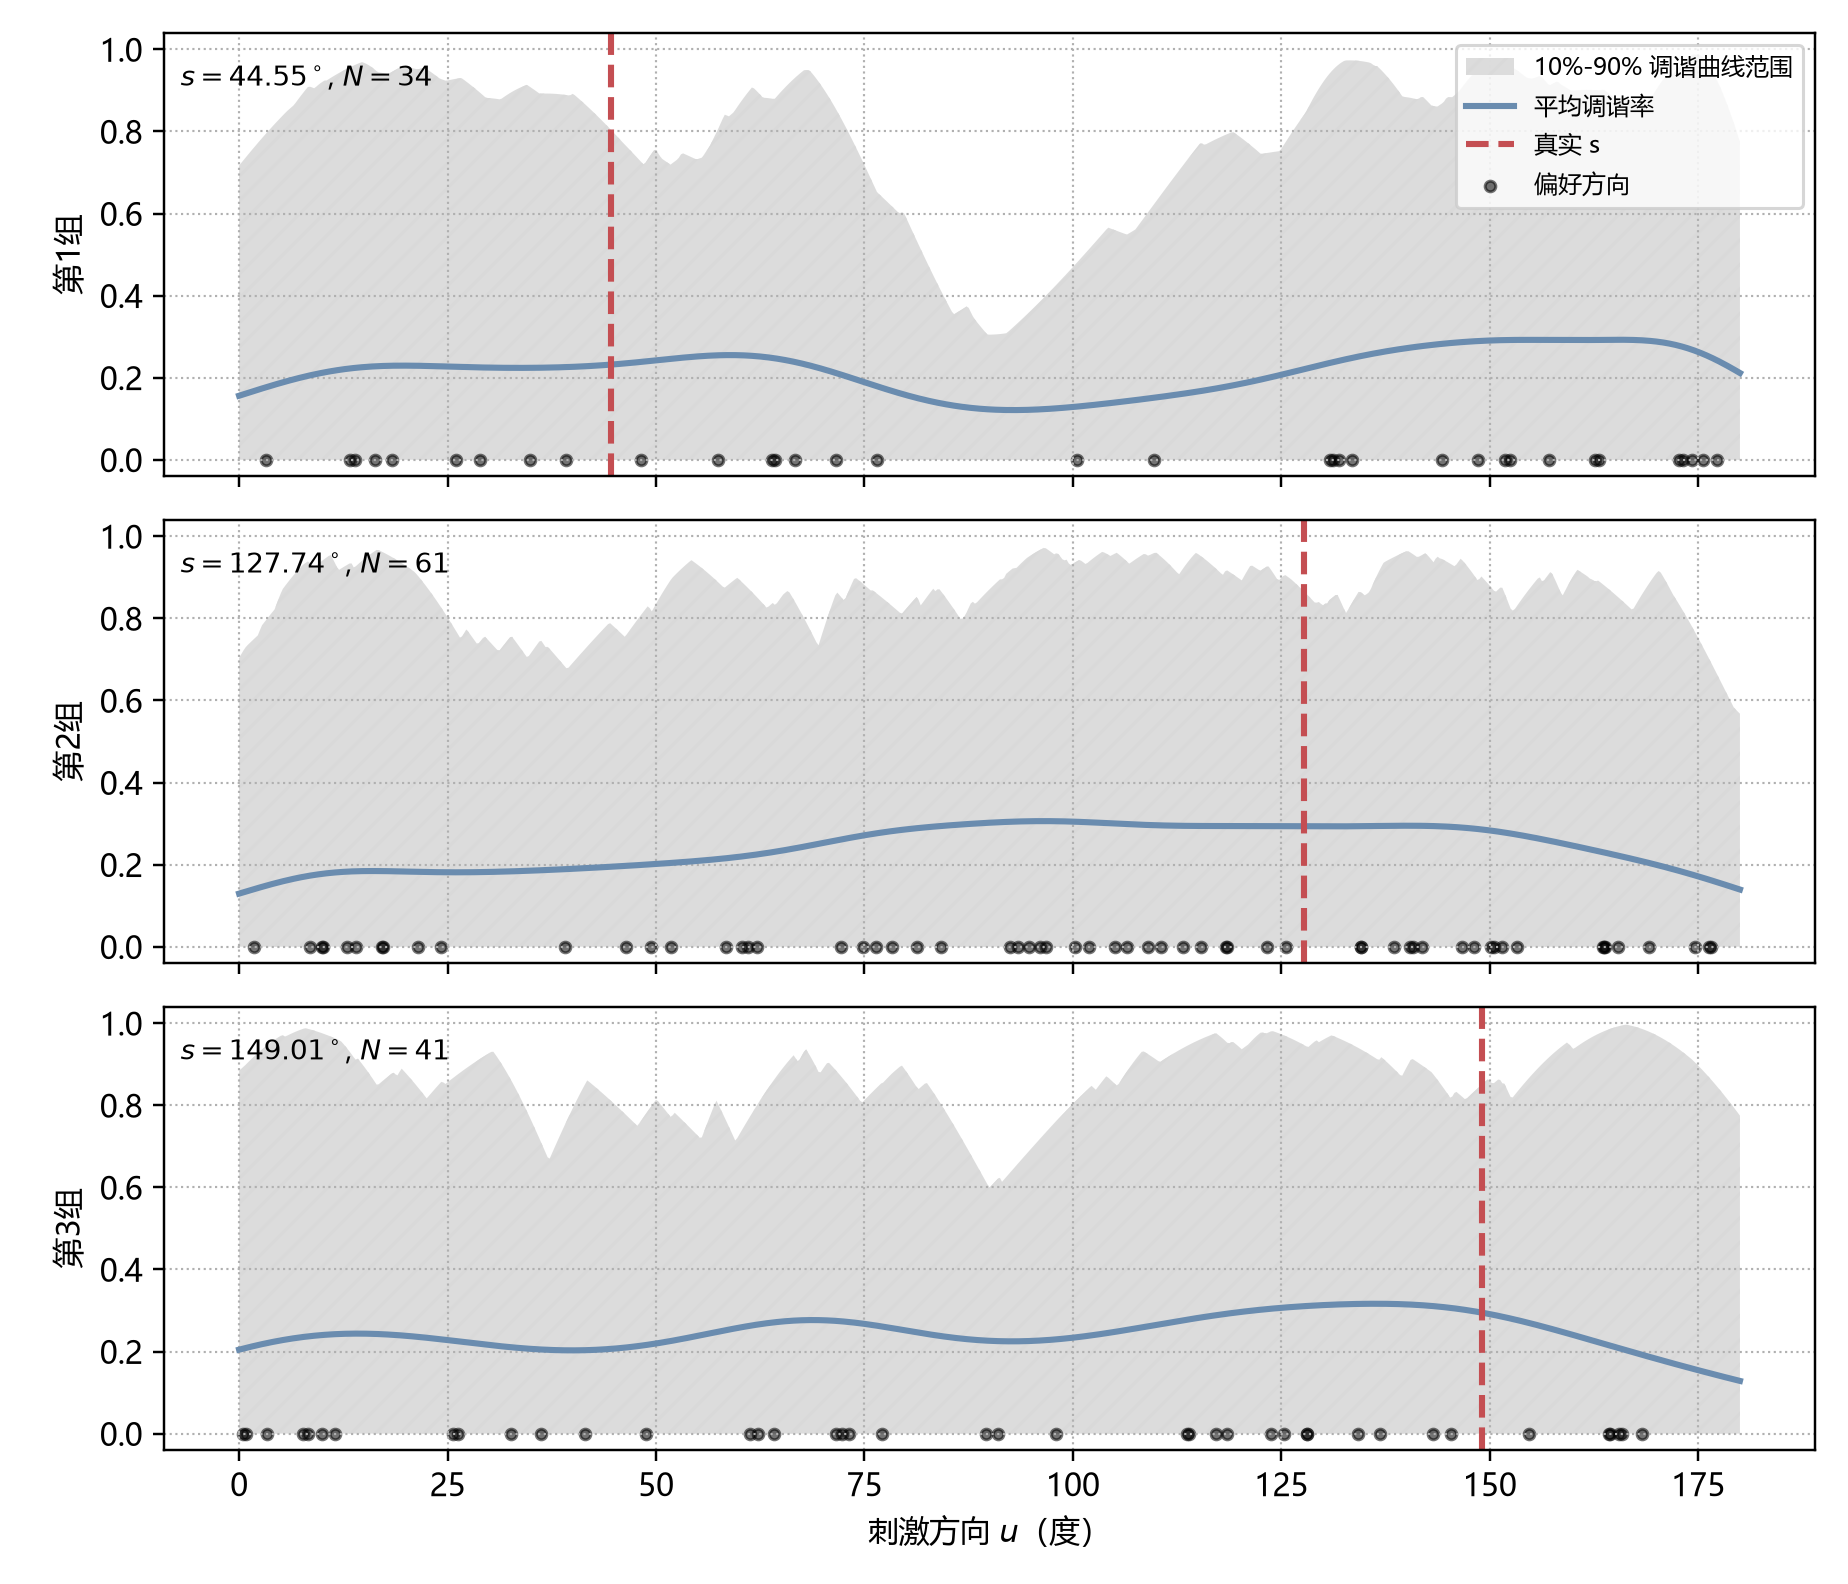
\includegraphics[width=0.88\textwidth]{python/Q4_outputs/random_parameter_sets.png}
\caption{第4题三组随机参数设置}
\label{fig:q4_random_parameters}
\end{figure}

图~\ref{fig:q4_random_parameters} 展示了三组随机生成的参数.灰色阴影表示所有神经元调谐曲线在每个刺激方向处的 \(10\%\)--\(90\%\) 分位范围, 蓝色曲线表示平均调谐率, 红色虚线表示真实刺激方向 \(s\), 底部黑点表示各神经元的偏好方向 \(s_a\).可以看出, 三组实验的真实方向, 神经元数目和偏好方向分布均不同, 因此可以检验估计方法在不同随机参数设置下的稳定性.

\begin{figure}[htbp]
\centering
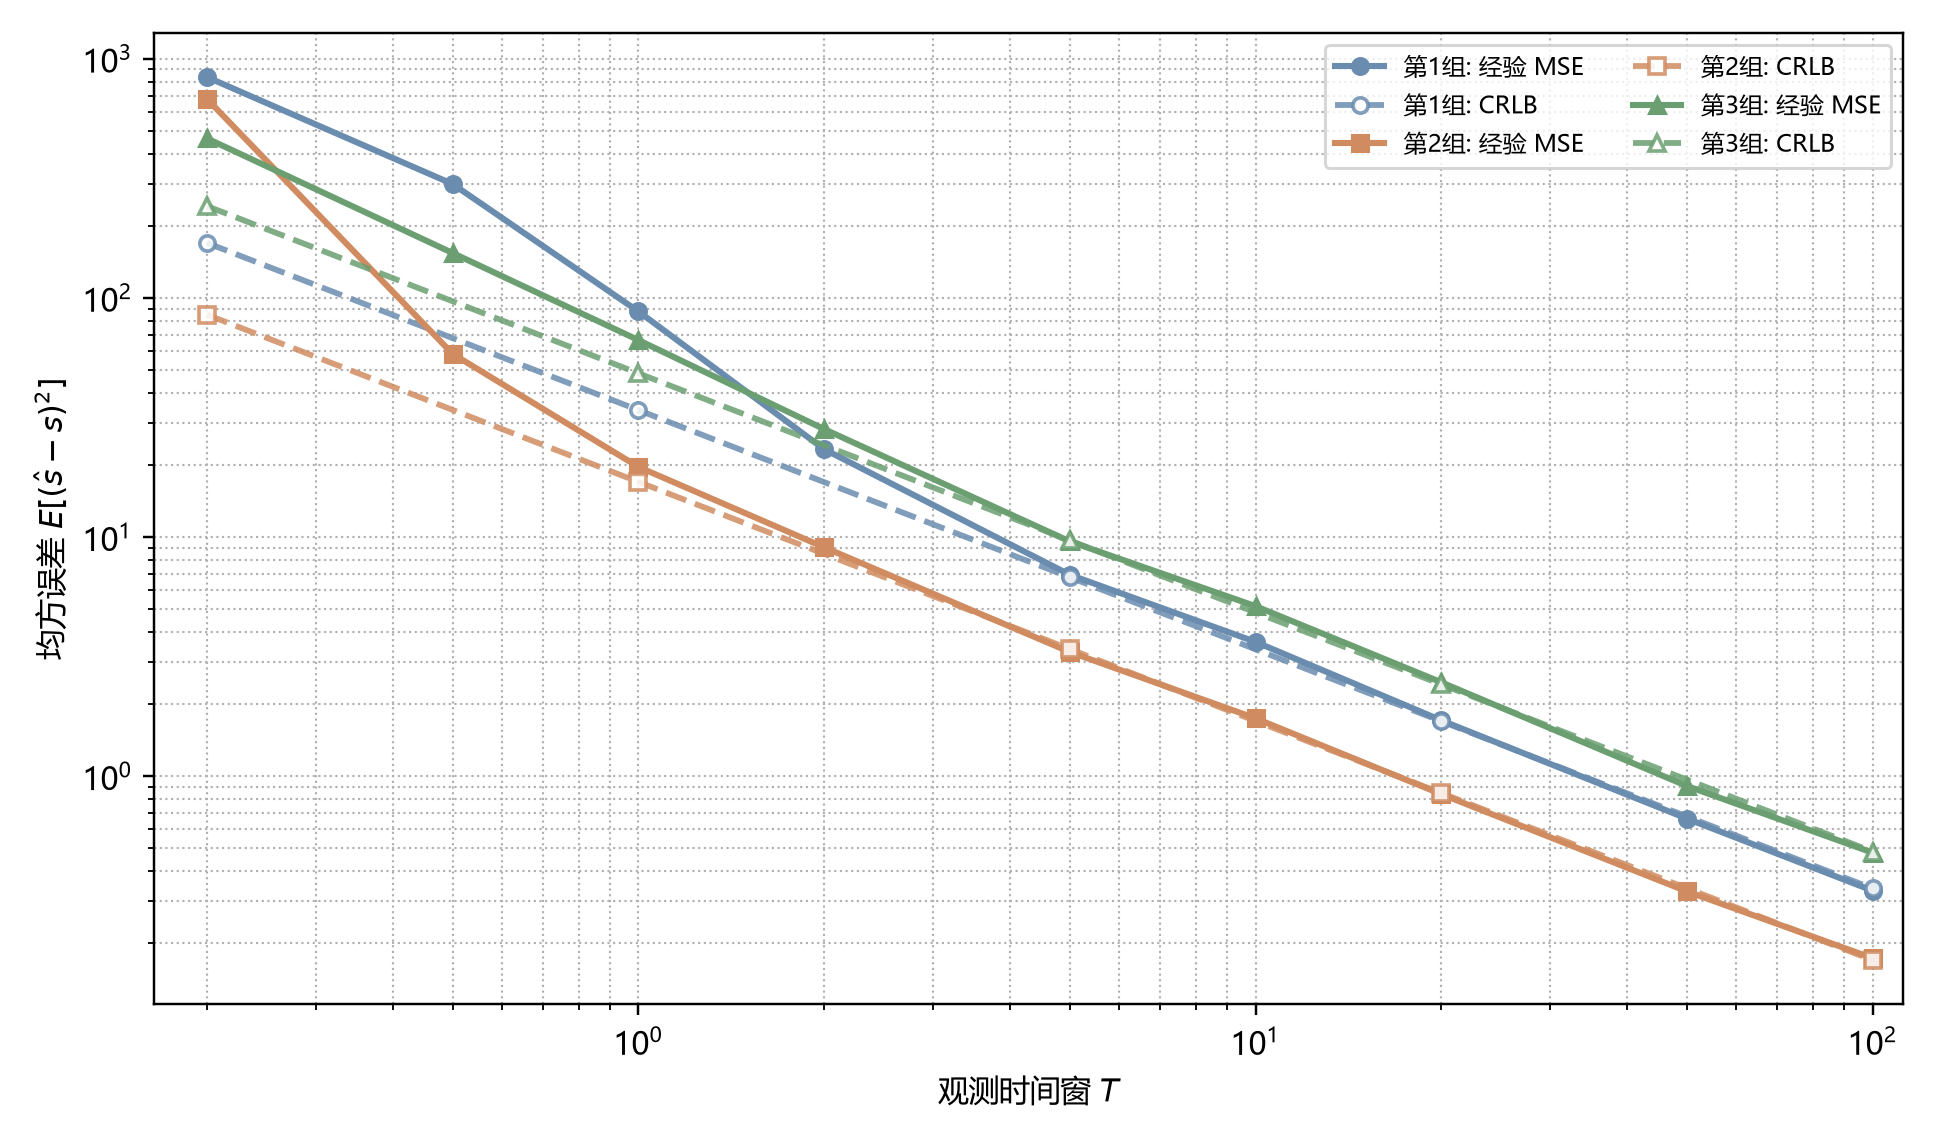
\includegraphics[width=0.88\textwidth]{python/Q4_outputs/mse_vs_time_window.png}
\caption{第4题不同时间窗下的经验 MSE 与 CRLB 对比}
\label{fig:q4_mse_crlb}
\end{figure}

图~\ref{fig:q4_mse_crlb} 给出了不同观测时间窗 \(T\) 下的误差结果.实线为经验 MSE, 虚线为空心标记的 CRLB.随着 \(T\) 增大, 泊松计数的平均发放次数增多, 观测数据包含的 Fisher 信息近似按 \(T\) 线性增加, 因此 CRLB 约按 \(1/T\) 下降.数值结果中, 经验 MSE 也随 \(T\) 增大而下降, 并且在较大的时间窗下逐渐接近对应的 CRLB, 这与前面关于 MLE 渐近有效性的推导一致.

\begin{figure}[htbp]
\centering
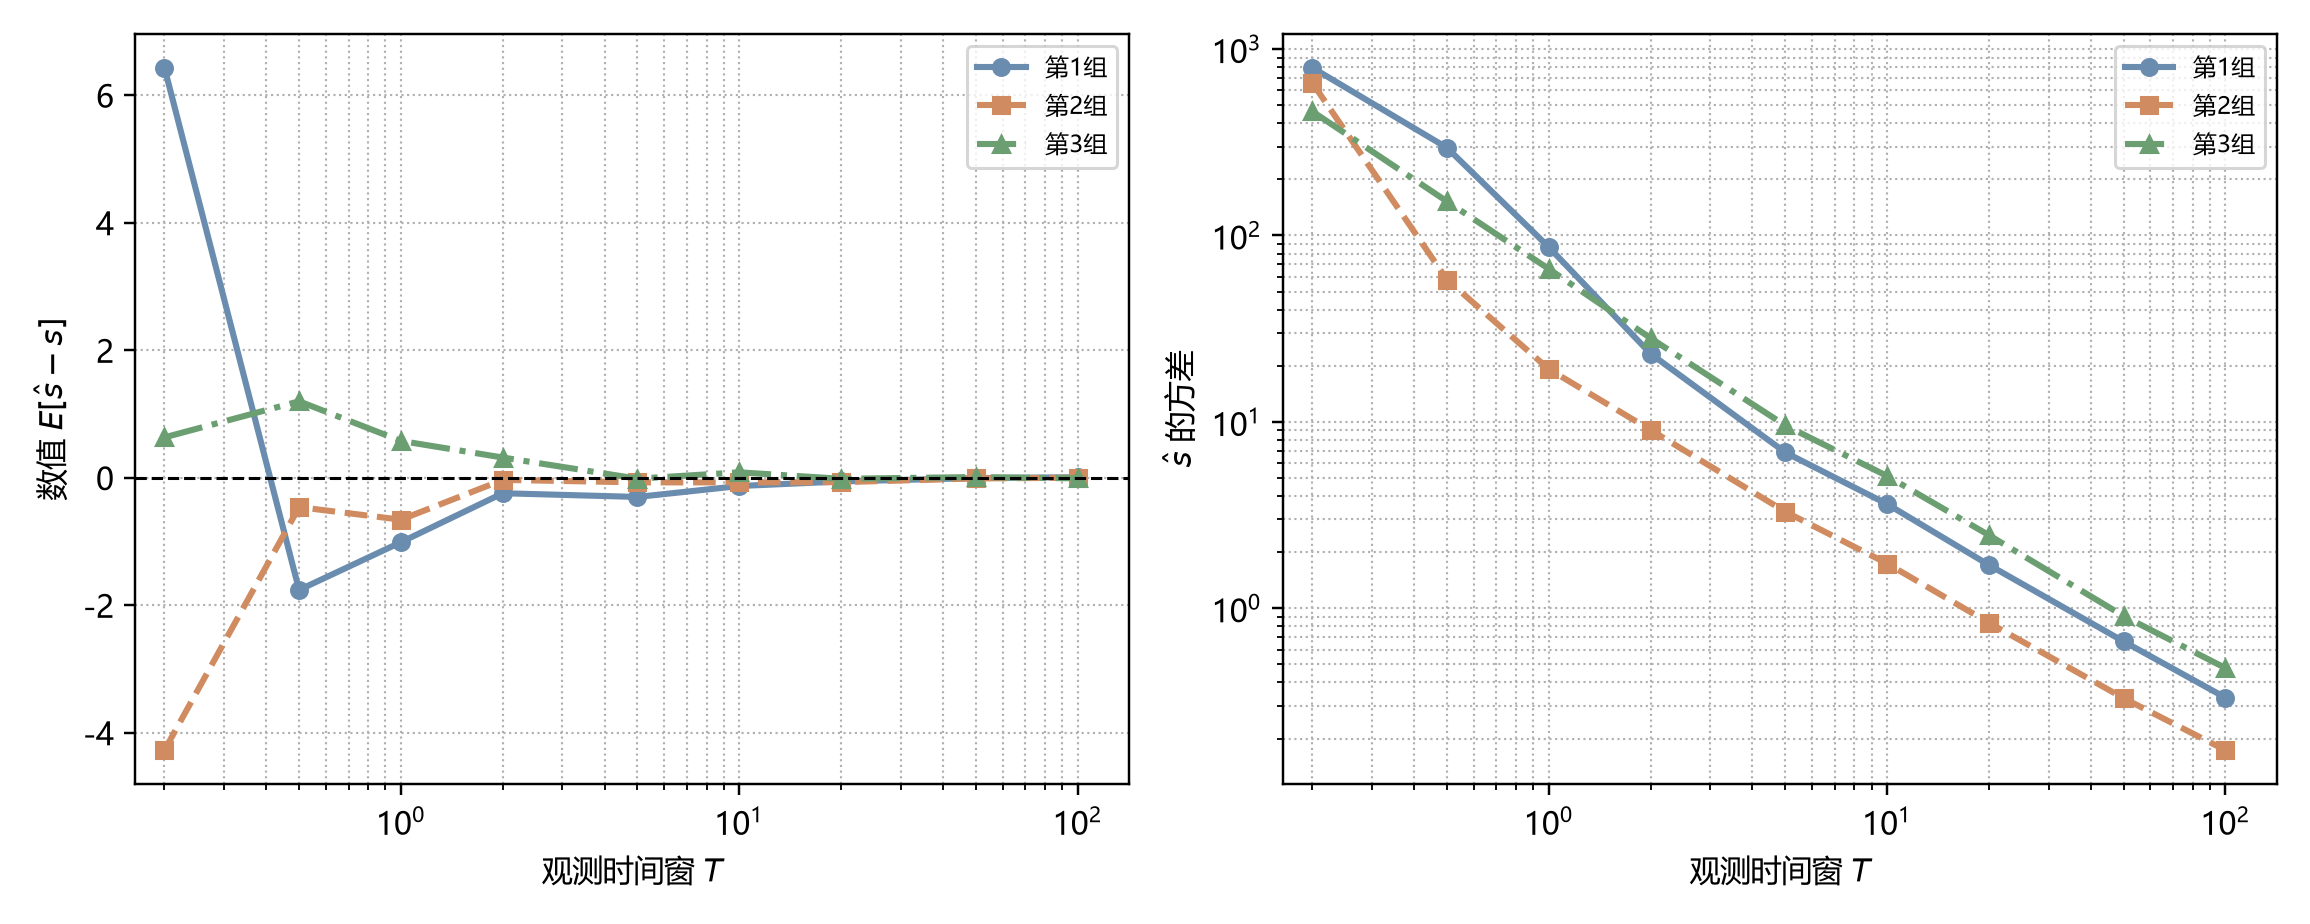
\includegraphics[width=0.92\textwidth]{python/Q4_outputs/bias_variance_vs_time_window.png}
\caption{第4题不同时间窗下的经验偏差与方差}
\label{fig:q4_bias_variance}
\end{figure}

图~\ref{fig:q4_bias_variance} 进一步将估计误差分解为偏差和方差两部分.左图中的经验偏差为 \(\mathbb E[\hat s-s]\), 右图为 \(\hat s\) 在重复实验中的经验方差.可以看到, 当 \(T\) 较小时, 泊松计数较少, 估计量可能有较明显偏差, 且不同重复实验之间波动较大;当 \(T\) 增大后, 三组实验的偏差整体趋近于 \(0\), 方差也明显下降.因此, 对于较大的观测时间窗, 有
\[
    \operatorname{MSE}(\hat s)
    =
    \operatorname{Var}(\hat s)
    +
    \operatorname{Bias}(\hat s)^2
    \approx
    \operatorname{Var}(\hat s), 
\]
结合图~\ref{fig:q4_mse_crlb} 中经验 MSE 接近 CRLB 的现象, 可以认为此时 MLE 已经接近无偏并接近理论下界, 数值实验表明其是渐近意义下 MVUB 估计的近似解.

\section{第5题}

程序
\texttt{python/Q5.py} 采用盲源分离处理该问题,  质量评价采用无参考指标,   并比较FastICA \cite{Hyvarinen1999FastICA} 和 AMUSE \cite{Tong1991Indeterminacy}两种方法.

\subsection{问题描述与混合模型}

设三路观测信号组成矩阵
\[
    X=
    \begin{bmatrix}
        x_1(1) & \cdots & x_1(T)\\
        x_2(1) & \cdots & x_2(T)\\
        x_3(1) & \cdots & x_3(T)
    \end{bmatrix}
    \in\mathbb R^{3\times T}.
\]
盲源分离的基本假设是
$X=A S$,  
其中 \(S\in\mathbb R^{3\times T}\) 是未知源信号,   \(A\) 是未知混合矩阵.目标是在不知道 \(A\) 和 \(S\) 的情况下估计一个解混矩阵 \(B\),  使
$\hat S=BX$
尽可能接近原始独立源信号.盲源分离本身只能确定源信号的排列,  符号和尺度到等价类,  因此程序最后会对每一路输出做标准化,  并按超额峰度大小给出确定的输出顺序.

预处理部分由函数\texttt{load\_bss\_audio},  \texttt{center\_rows} 和 \texttt{whiten\_rows} 完成,  核心步骤如下.

\begin{enumerate}
    \item 读取附件中的 wav 文件,  将 PCM 音频转换为浮点数并归一化到 \([-1,  1]\);若音频为多声道,  则先取声道平均得到单声道信号.
    \item 检查所有混合信号的采样率是否一致,  并截断到相同长度,  然后按行堆叠成矩阵 \(X\).
    \item 对每一路信号去均值,   即$X_c=X-\bar X$.
    \item 对中心化后的数据白化.令$C_x=\frac{1}{T}X_cX_c^\top=E\Lambda E^\top$,  
    其中 \(\Lambda\) 是特征值对角矩阵,  \(E\) 是特征向量矩阵.程序使用$
        Z=\Lambda^{-1/2}E^\top X_c$
    得到白化信号 \(Z\),  使 \(\frac{1}{T}ZZ^\top\approx I\). \textbf{后续分离问题可以转化为寻找一个正交分离矩阵} $W$,  \textbf{使得}$WZ$\textbf{中的各行分量尽可能相互独立}.
\end{enumerate}

\subsection{算法一: FastICA}

FastICA 的思想是利用``独立源信号通常比其线性混合更非高斯"这一假设.程序中的 \texttt{fastica} 函数采用对称 FastICA \cite{Hyvarinen1999FastICA},  并使用 \(\tanh\) 非线性函数作为近似负熵的对比函数.白化后设分离矩阵为 \(W\),  输出为
\(Y=WZ\).
每次迭代先计算
\(g(Y)=\tanh(Y)\),  \(g'(Y)=1-\tanh^2(Y)\).
对称 FastICA 的固定点更新在程序中写为
\begin{equation}
    W_{\mathrm{new}}
    =
    \frac{1}{T}g(WZ)Z^\top
    -
    \operatorname{diag}
    \left(
        \frac{1}{T}\sum_{t=1}^T g'(Y(:,  t))
    \right)W.
\end{equation}
为了避免不同分量收敛到同一个方向,  每次更新后通过奇异值分解做对称去相关(即首先设$W_{\mathrm{new}}=U\Sigma V^\top$,  然后令$W_{\mathrm{new}}=UV^\top$).
停止准则为相邻两次迭代方向几乎不再变化,  即
\(\max_i\left||w_i^{(k+1)\top}w_i^{(k)}|-1\right|<10^{-6}\).

\subsection{算法二: AMUSE}

AMUSE(Algorithm for Multiple Unknown Signals Extraction)主要利用源信号的时间相关结构 \cite{Tong1991Indeterminacy}.它在白化后寻找一个旋转,  使带延迟协方差矩阵尽量对角化.对给定延迟 \(\tau\),  程序先计算
\begin{equation}
    C_\tau
    =
    \frac{1}{T-\tau}Z_{:,  \tau+1: T}Z_{:,  1: T-\tau}^{\top},  
\end{equation}
并取对称部分
\(\widetilde C_\tau=\frac{1}{2}(C_\tau+C_\tau^\top)\).
然后对 \(\widetilde C_\tau\) 做特征分解.若
\(\widetilde C_\tau=QDQ^\top\),  
则用
\(\hat S=Q^\top Z\)
作为该延迟下的分离结果.直观上,  如果不同源信号在延迟 \(\tau\) 下互不相关,  那么正确的旋转应当让延迟协方差矩阵的非对角项接近 \(0\).

由于音频信号的有效时间尺度未知,  程序尝试
\[\tau\in\{1,  2,  4,  8,  16,  32,  64,  128,  0.005f_s,  0.010f_s,  0.020f_s,  0.040f_s\},  \]
其中 \(f_s\) 是采样率.对每个候选延迟运行一次 AMUSE,  再用多个短延迟下的平均非对角时间协方差作为盲评价准则,  选择得分最小的延迟.

\subsection{伪代码}

程序 \texttt{python/Q5.py} 核心伪代码如算法~\ref{alg:q5} 所示.

\begin{algorithm}[htbp]
\caption{第5题盲源分离实验流程}
\label{alg:q5}
\small
\begin{algorithmic}[1]
\Require 三路混合音频文件集合 \(\mathcal D\),  FastICA 随机种子 \(r\)
\Ensure FastICA 与 AMUSE 的分离信号,  无参考评价指标和可视化结果
\State 读入所有 wav 文件,  转换为单声道浮点信号,  并检查采样率一致性
\State 截断到相同长度,  将三路混合信号堆叠为观测矩阵 \(X\in\mathbb R^{3\times T}\)
\State 对 \(X\) 去均值并白化,  得到 \(Z=\Lambda^{-1/2}E^\top(X-\bar X)\)
\Statex
\State \textbf{FastICA 分离}
\State 随机初始化分离矩阵 \(W\),  并做对称去相关
\Repeat
    \State \(Y\gets WZ\)
    \State \(G\gets \tanh(Y)\),  \(d\gets \operatorname{mean}(1-\tanh^2(Y))\)
    \State \(W_{\rm new}\gets GZ^\top/T-\operatorname{diag}(d)W\)
    \State 对 \(W_{\rm new}\) 做对称去相关
    \State \(\Delta\gets \max_i\left||w_i^{\rm new\top}w_i|-1\right|\)
    \State \(W\gets W_{\rm new}\)
\Until{\(\Delta<\varepsilon\) 或达到最大迭代次数}
\State \(\hat S_{\rm ICA}\gets WZ\),  并对输出做标准化,  符号修正和排序
\Statex
\State \textbf{AMUSE 分离}
\State 设候选延迟集合 \(\mathcal L_1=\{1,  2,  4,  8,  16,  32,  64,  128\}\)
\State 设音频尺度延迟集合 \(\mathcal L_2=\{0.005f_s,  0.010f_s,  0.020f_s,  0.040f_s\}\)
\State \(\mathcal L\gets\mathcal L_1\cup\mathcal L_2\)
\ForAll{\(\tau\in\mathcal L\)}
    \State \(C_\tau\gets Z_{:,  \tau+1: T}Z_{:,  1: T-\tau}^{\top}/(T-\tau)\)
    \State \(\widetilde C_\tau\gets (C_\tau+C_\tau^\top)/2\)
    \State 对 \(\widetilde C_\tau\) 做特征分解,  取旋转矩阵 \(Q_\tau\)
    \State \(\hat S_\tau\gets Q_\tau^\top Z\),  并计算时间协方差非对角得分 \(J(\tau)\)
\EndFor
\State 取 \(\tau^*=\arg\min_{\tau\in\mathcal L}J(\tau)\),  令 \(\hat S_{\rm AMUSE}\gets\hat S_{\tau^*}\)
\Statex
\ForAll{\(S\in\{X,  \hat S_{\rm ICA},  \hat S_{\rm AMUSE}\}\)}
    \State 计算平均绝对相关系数,  归一化互信息,  时间协方差非对角项和平均绝对超额峰度
\EndFor
\State 保存分离音频,  指标表,  波形图和指标柱状图
\end{algorithmic}
\end{algorithm}

\subsection{质量评价指标}

由于附件未提供参考源信号,  因此程序使用以下指标平均绝对相关系数、成对归一化互信息、时间协方差非对角项和平均绝对超额峰度来比较混合信号、 FastICA 输出和 AMUSE 输出. 相关指标的计算方法和判读方式如表~\ref{tab:q5_metric_definitions} 所示.

\begin{table}[htbp]
\centering
\caption{第5题无参考质量评价指标}
\label{tab:q5_metric_definitions}
\renewcommand{\arraystretch}{1.16}
\begin{tabular}{@{}>{\raggedright\arraybackslash}p{0.20\textwidth}
                  >{\raggedright\arraybackslash}p{0.51\textwidth}
                  >{\raggedright\arraybackslash}p{0.22\textwidth}@{}}
\toprule
指标 & 计算方法 & 判读方式 \\
\midrule
平均绝对相关系数
& 对标准化后的各路信号计算相关系数矩阵, 取非对角元素绝对值的平均.
& 越小表示不同分离分量的线性相关越弱. \\
成对归一化互信息
& 用二维直方图估计每对分量的互信息, 并除以边缘熵的几何平均进行归一化.
& 越小表示统计依赖越弱. \\
时间协方差非对角项
& 对若干延迟计算跨通道延迟协方差的非对角元素平均绝对值.
& 越小表示分离后的源信号在时间结构上越接近互不相关. \\
平均绝对超额峰度
& 语音, 音乐等真实音频源通常具有明显非高斯性, 因此分离后该值往往比混合信号更大.
& 可辅助判断分离是否提取出了更尖峰, 更稀疏的源结构. \\
\bottomrule
\end{tabular}
\end{table}

\subsection{实验结果与分析}

程序将分离后的音频保存到 \texttt{python/Q5\_outputs/} 下的 \texttt{fastica} 和 \texttt{amuse} 子目录,  并输出波形图、指标图和 \texttt{quality\_metrics.csv}.本次运行得到的主要质量指标如表~\ref{tab:q5_metrics}, 图~\ref{fig:q5_waveforms} 和图~\ref{fig:q5_quality_metrics} 所示.

\begin{figure}[htbp]
    \centering
    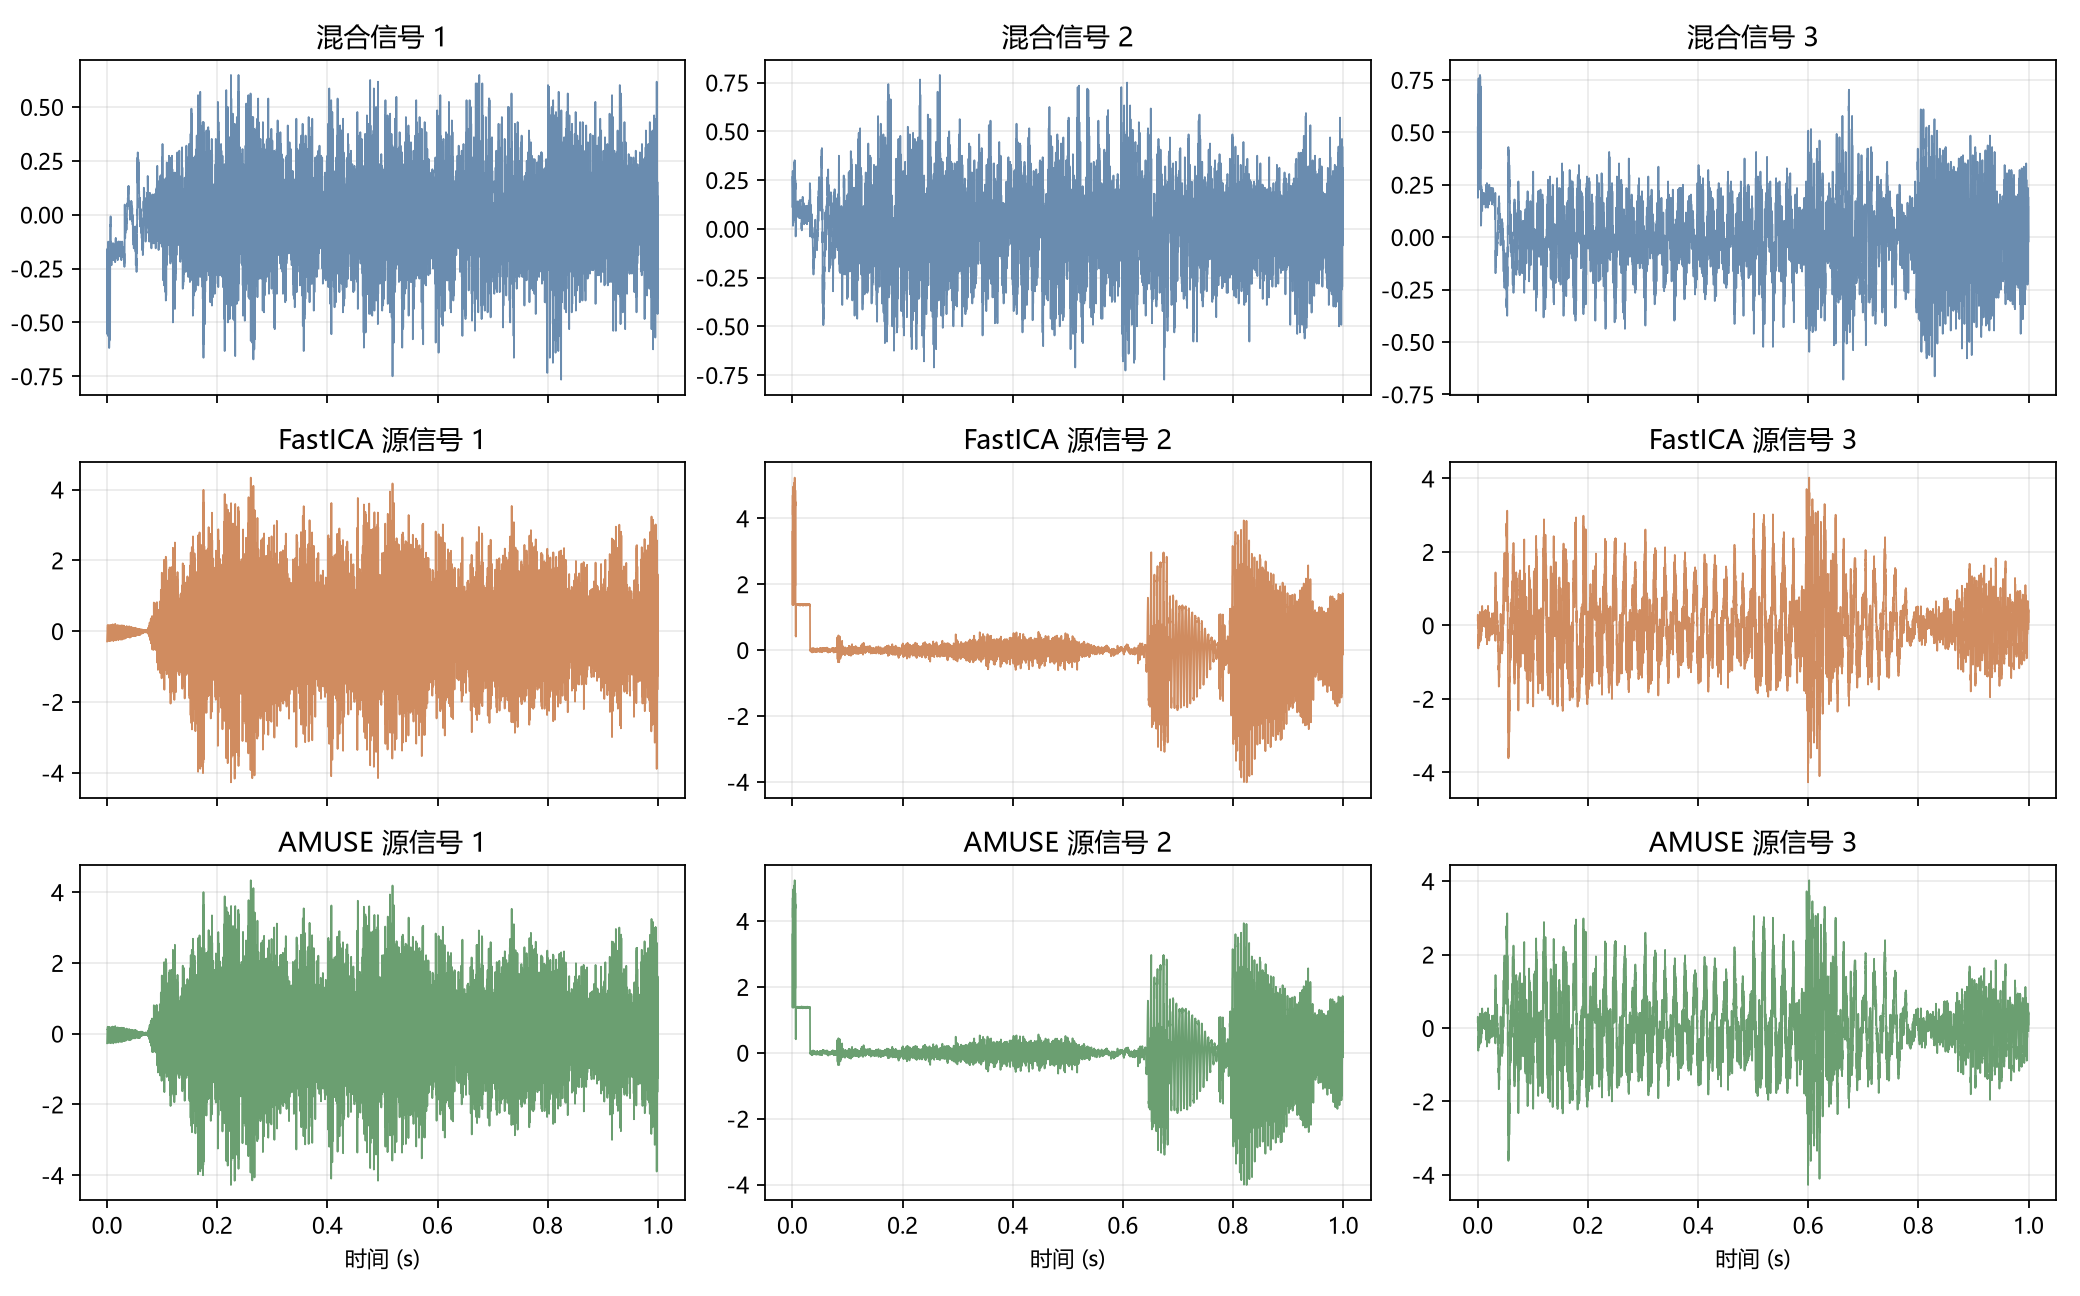
\includegraphics[width=0.95\textwidth]{python/Q5_outputs/waveforms.png}
    \caption{第5题混合信号与分离信号波形对比}
    \label{fig:q5_waveforms}
\end{figure}

\begin{figure}[htbp]
    \centering
    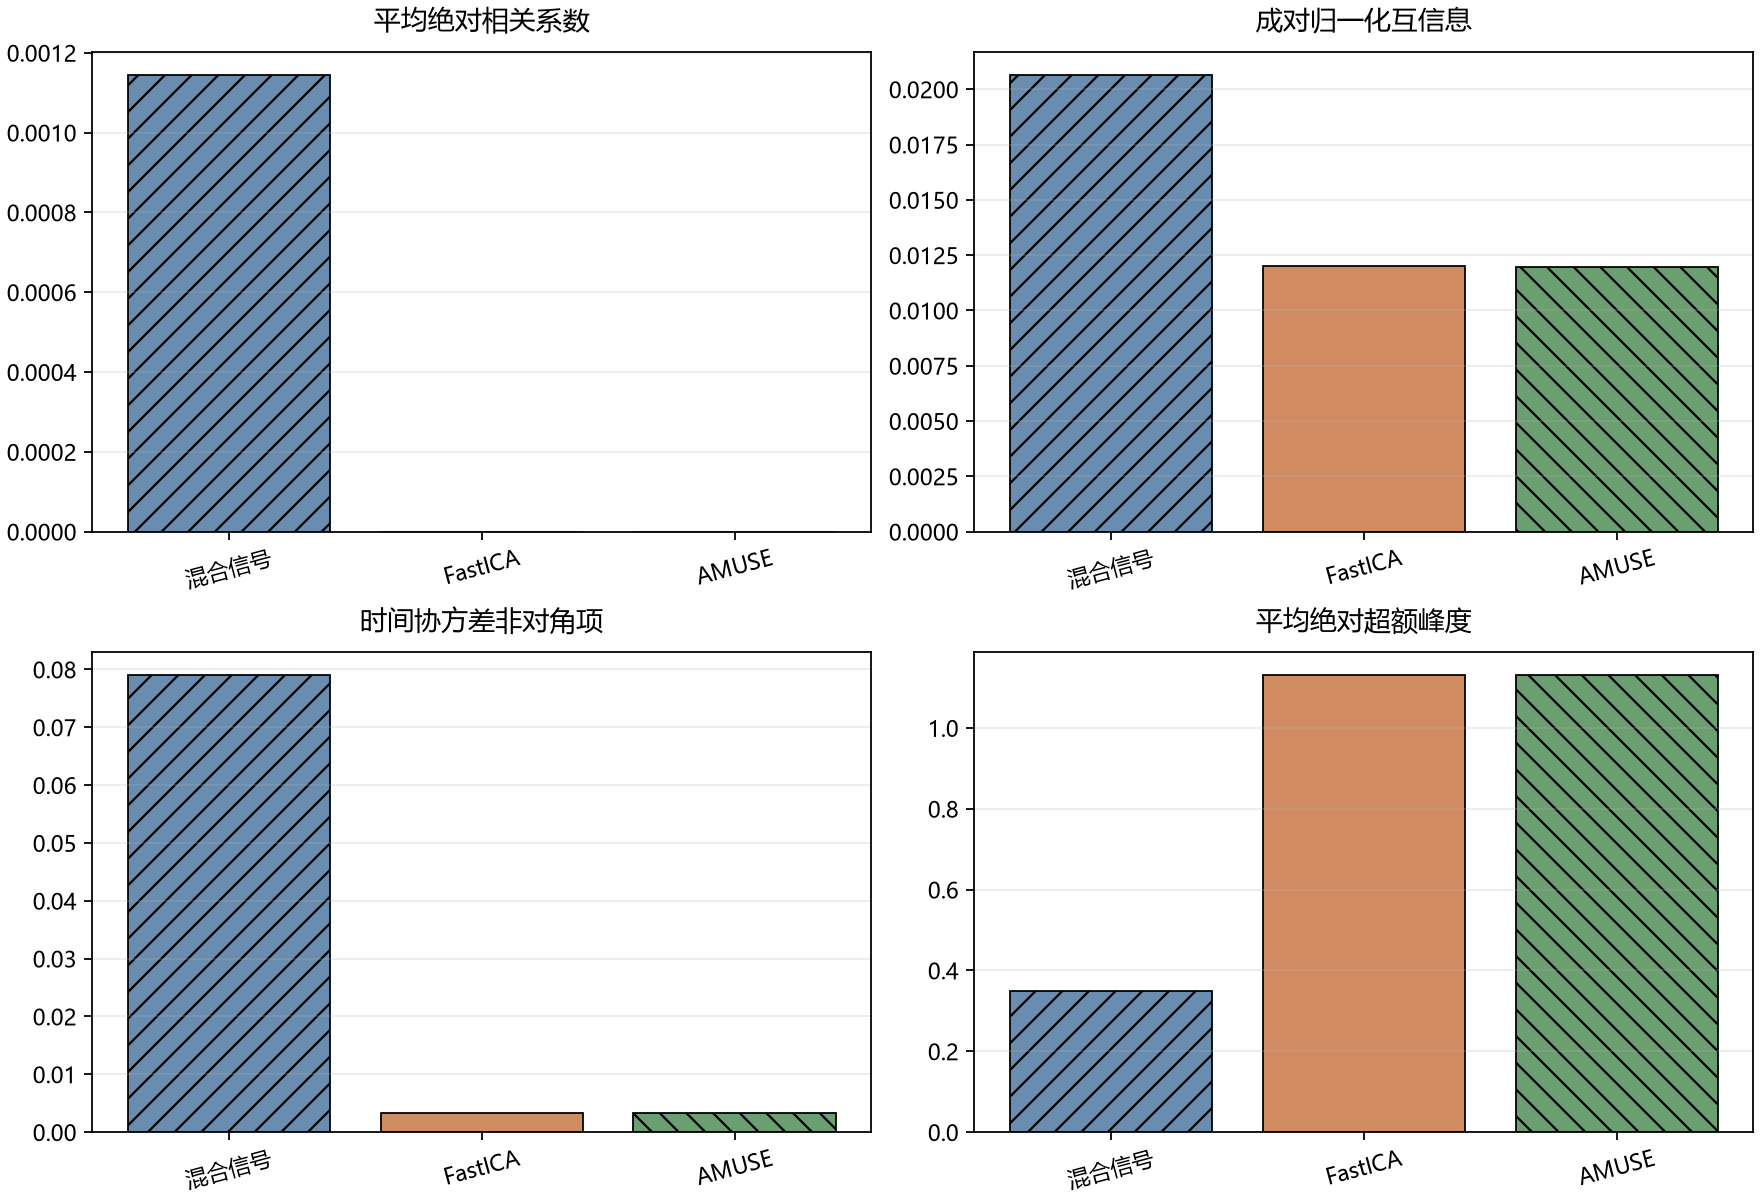
\includegraphics[width=0.85\textwidth]{python/Q5_outputs/quality_metrics.png}
    \caption{第5题无参考质量指标对比}
    \label{fig:q5_quality_metrics}
\end{figure}

\begin{table}[htbp]
\centering
%\scriptsize
\caption{第5题实验结果}
\label{tab:q5_metrics}
\begin{tabular}{lcccc}
\toprule
方法
& 平均相关
& 成对归一化
& 时间非对角
& 平均超额峰度
\\
\midrule
混合信号
& \(1.145\times10^{-3}\)
& \(2.0656\times10^{-2}\)
& \(7.8991\times10^{-2}\)
& \(3.48715\times10^{-1}\)
\\
FastICA
& \(2.12\times 10^{-16}\)
& \(1.2023\times10^{-2}\)
& \(3.381\times10^{-3}\)
& \(1.130283\times10^{0}\)
\\
AMUSE
& \(2.91\times 10^{-16}\)
& \(1.1950\times10^{-2}\)
& \(3.244\times10^{-3}\)
& \(1.129892\times10^{0}\)
\\
\bottomrule
\end{tabular}
\end{table}

可以看到,  两种算法都显著降低了分量之间的归一化互信息和时间协方差非对角项,  同时使平均绝对超额峰度明显增大,  说明分离后的信号比原始混合信号更接近相互独立的非高斯源信号. FastICA 和 AMUSE 在该数据上的表现非常接近; AMUSE 的时间协方差非对角项和互信息略低,  说明它对这组音频的时间相关结构利用得稍好; FastICA 的结果也已经达到接近零相关的效果,  说明基于非高斯性的独立成分分解同样适合本题.

\section{第6题}

\subsection{实验任务与网络结构}

本题程序 \texttt{python/Q6.py} 在 MNIST 手写数字数据集上训练同一个多层感知机,  并比较普通带动量随机梯度下降
(SGD with momentum)与阻尼小批量自然梯度(damped mini-batch Natural Gradient,   NG)的训练效果.输入图像先做标准化,  
为了方便代码实现,  这里使用MLP,  网络结构为
\[
    784(28\times28\text{个输入特征}) \longrightarrow 128 \longrightarrow 64 \longrightarrow 10,  
\]
隐藏层使用 ReLU,  输出层使用 softmax 交叉熵损失.该网络共有 \(109386\) 个可训练参数,  如果显式保存完整 Fisher 矩阵,  
仅 float32 存储就约需要 \(44.6\) GiB,  因此程序使用 Fisher向量逐点相乘与共轭梯度法近似求自然梯度方向.

\subsection{核心实现思路与伪代码}

SGD 部分直接使用 PyTorch 的 \texttt{torch.optim.SGD},  学习率为 \(0.10\),  动量为 \(0.90\).自然梯度部分的核心是求解
\[
    (F+\lambda I)d=\nabla_\theta L(\theta),  
\]
其中 \(F\) 为 Fisher 信息矩阵,  \(\lambda=0.10\) 为阻尼系数.得到方向 \(d\) 后按
$
    \theta \leftarrow \theta-\eta d
$
更新参数,  实验中自然梯度学习率取 \(\eta=0.05\).为避免显式构造 \(F\),  代码把 Fisher 近似为
$
    \operatorname{KL}\!\left(p_{\theta_{\rm old}}(\cdot|x)\,  \|\,  p_\theta(\cdot|x)\right)
$
在当前参数处的 Hessian,  并通过二阶自动微分计算 \((F+\lambda I)v\),  再用共轭梯度法求解线性方程.

核心伪代码如算法~\ref{alg:q6} 所示.

\begin{algorithm}[htbp]
\caption{第6题 SGD 与阻尼自然梯度训练流程}
\label{alg:q6}
\small
\begin{algorithmic}[1]
\Require MNIST 训练集与测试集,  训练轮数 \(E\),  阻尼系数 \(\lambda\),  自然梯度学习率 \(\eta_{\rm NG}\)
\Ensure 两种优化方法的训练损失,  测试损失,  训练准确率和测试准确率
\State 固定随机种子,  读取并标准化 MNIST 数据
\State 构造 MLP:\(784\to128\to64\to10\),  保存初始参数 \(\theta_0\)
\ForAll{\(m\in\{\mathrm{SGD},  \mathrm{NG}\}\)}
    \State 重置模型参数 \(\theta\gets\theta_0\),  并使用相同的数据打乱顺序
    \For{\(e=1,  \ldots,  E\)}
        \ForAll{mini-batch \((x,  y)\)}
            \State \(\ell(\theta)\gets \operatorname{CE}(f_\theta(x),  y)\)
            \If{\(m=\mathrm{SGD}\)}
                \State 反向传播得到梯度 \(\nabla_\theta\ell\)
                \State 用带动量 SGD 更新 \(\theta\)
            \Else
                \State \(g\gets \operatorname{vec}(\nabla_\theta\ell)\)
                \State 固定 \(p_{\rm old}=\operatorname{softmax}(f_\theta(x))\)
                \Function{Avp}{$v$}
                    \State \(D_{\rm KL}\gets {\rm KL}\left(p_{\rm old}\,  \|\,  \operatorname{softmax}(f_\theta(x))\right)\)
                    \State \(h\gets \nabla_\theta^2D_{\rm KL}\,  v\)
                    \State \Return \(h+\lambda v\)
                \EndFunction
                \State 用共轭梯度近似求解 \(\operatorname{Avp}(d)=g\)
                \State 若 \(\|d\|\) 超过阈值,  则对 \(d\) 做范数裁剪
                \State \(\theta\gets\theta-\eta_{\rm NG}d\)
            \EndIf
        \EndFor
        \State 在训练集和测试集上计算损失与准确率
    \EndFor
\EndFor
\State 保存 CSV 结果并绘制准确率,  损失曲线
\end{algorithmic}
\end{algorithm}

\subsection{实验结果与分析}

实验使用完整 MNIST 训练集,  batch size 为 \(512\),  测试 batch size 为 \(1024\),  训练 \(5\) 个 epoch.固定随机种子为 \(42\),  
并让两种方法使用相同的网络初值和相同的数据打乱顺序.程序输出结果保存在
\texttt{python/Q6\_outputs/sgd\_vs\_ng\_results.csv},  同时生成准确率曲线和损失曲线.

\begin{figure}[htbp]
\centering
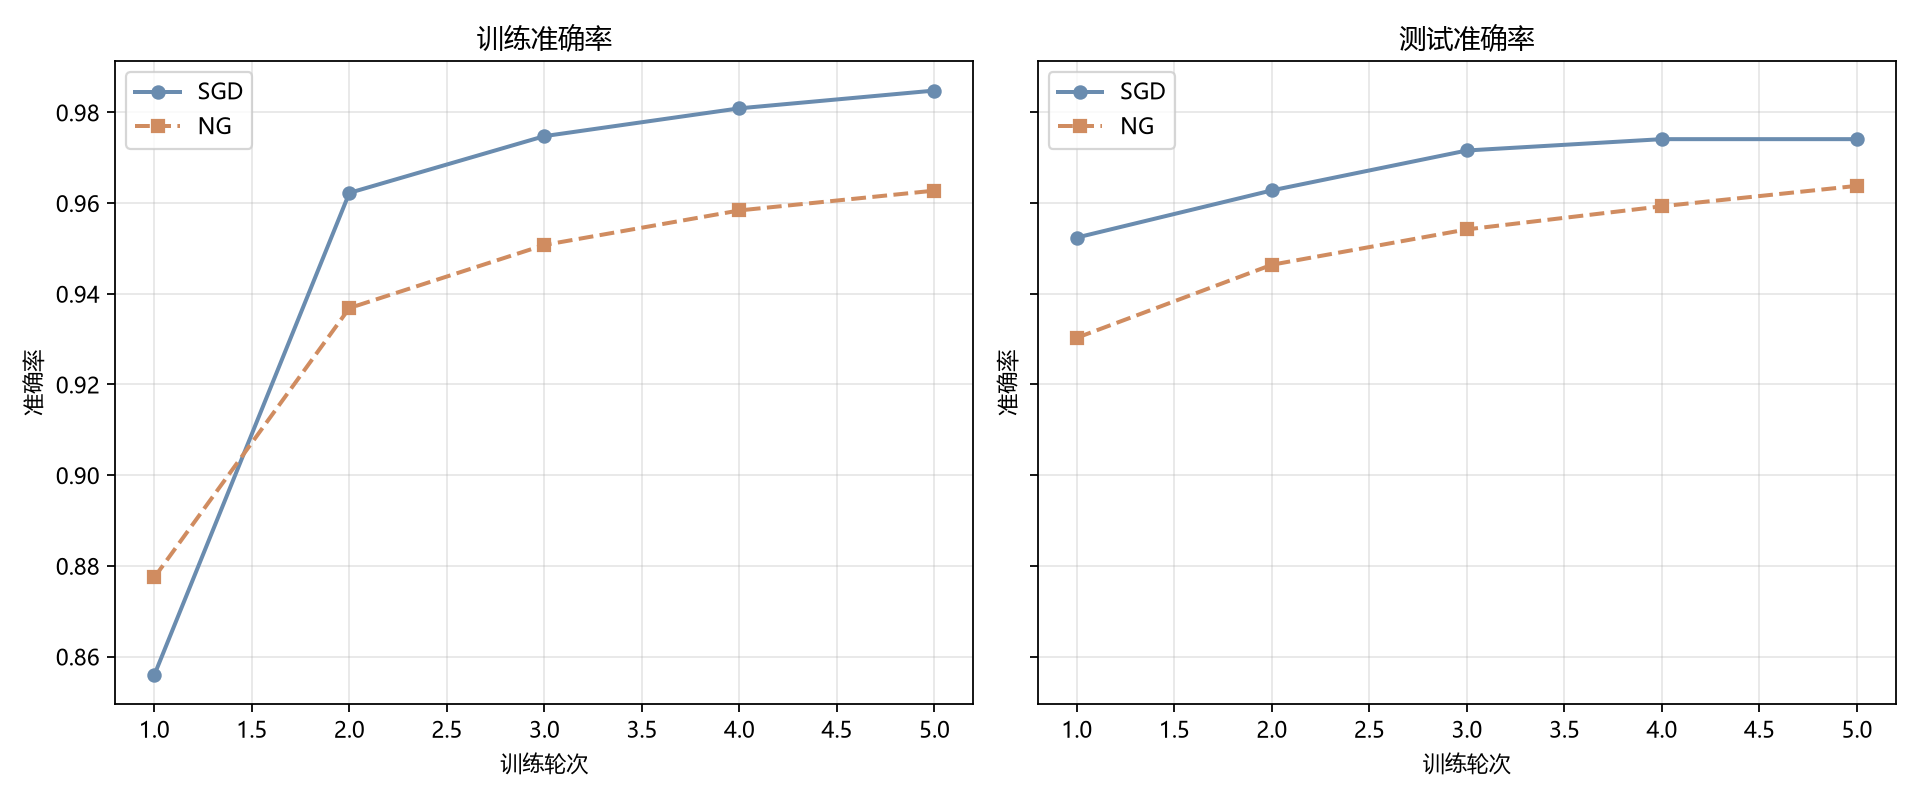
\includegraphics[width=0.82\textwidth]{python/Q6_outputs/accuracy_comparison.png}
\caption{第6题准确率曲线}
\label{fig:q6_accuracy}
\end{figure}

\begin{figure}[htbp]
\centering
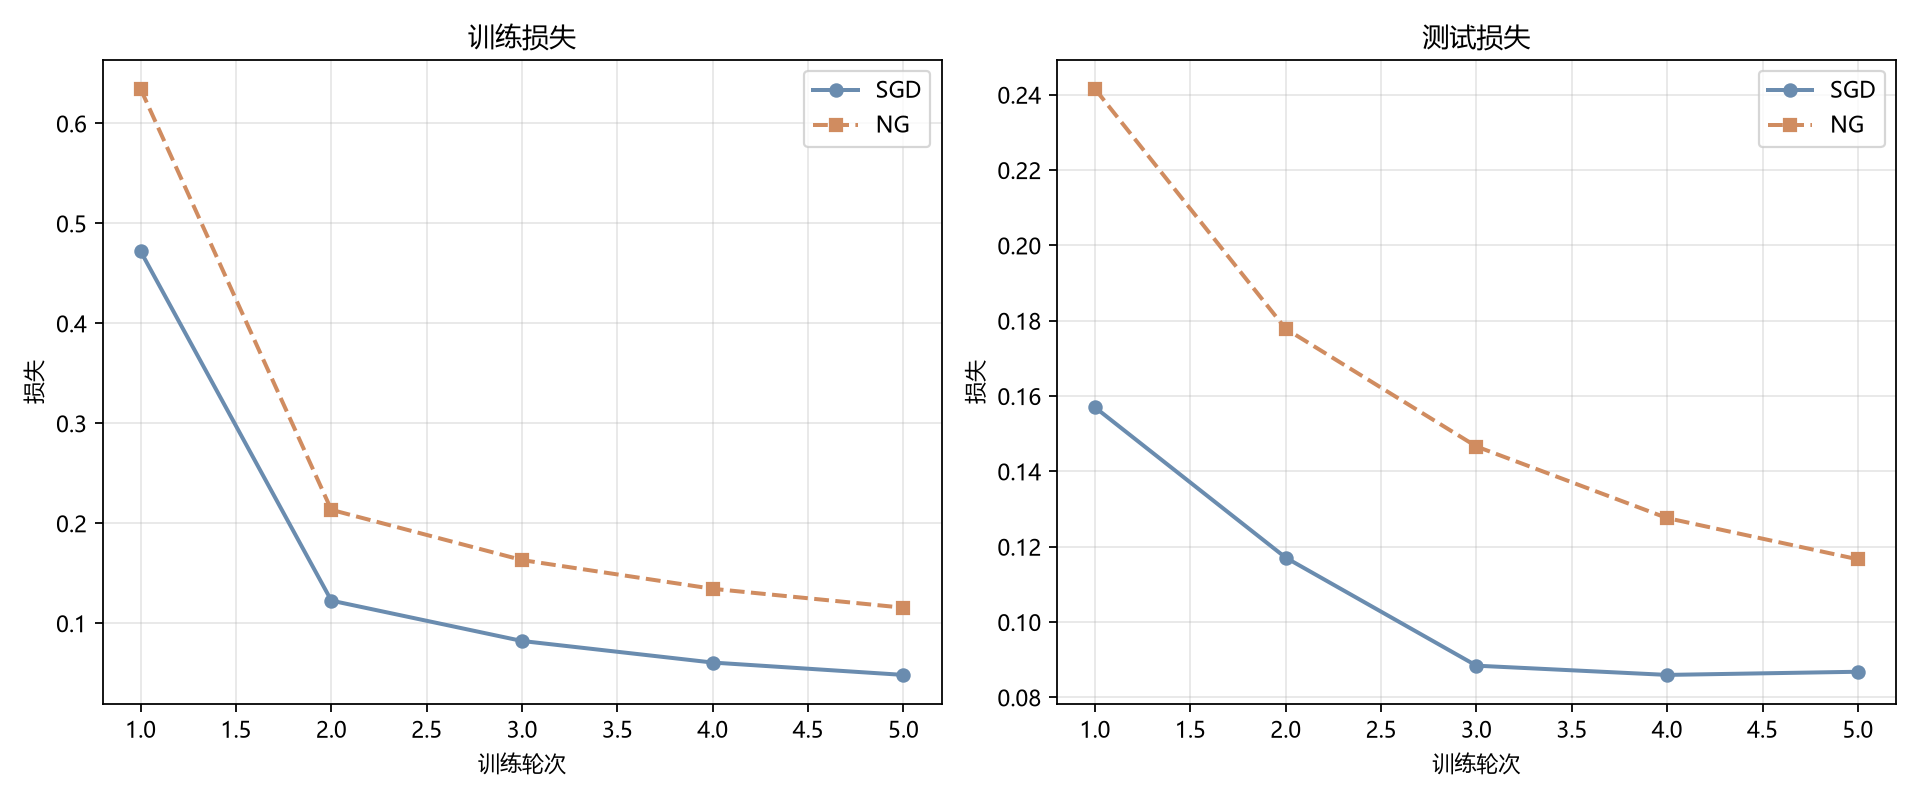
\includegraphics[width=0.82\textwidth]{python/Q6_outputs/loss_comparison.png}
\caption{第6题损失曲线}
\label{fig:q6_loss}
\end{figure}

\begin{table}[htbp]
\centering
%\scriptsize
\caption{第6题实验结果}
\label{tab:q6_results}
\begin{tabular}{lccccc}
\toprule
方法
& Test acc@1
& Train acc@5
& Test acc@5
& Test loss@5
& 总耗时/s
\\
\midrule
SGD
& 0.9524
& 0.9848
& 0.9741
& 0.0868
& 145.76
\\
NG
& 0.9303
& 0.9628
& 0.9638
& 0.1167
& 150.35
\\
\bottomrule
\end{tabular}
\end{table}

从结果可以看出(见表~\ref{tab:q6_results},  图~\ref{fig:q6_accuracy},  图~\ref{fig:q6_loss}),  在本次超参数设置下,  SGD 的收敛速度和最终测试准确率都略优于自然梯度. SGD 在第 \(1\) 轮就达到
\(95.24\%\) 的测试准确率,  第 \(5\) 轮达到 \(97.41\%\);自然梯度从 \(93.03\%\) 提升到 \(96.38\%\),  也能稳定收敛,  
但最终精度略低.造成这种现象的主要原因是自然梯度实现中使用的是阻尼 Fisher 近似,  并且每个 batch 只用 \(8\) 次共轭梯度迭代,  
因此求得的是近似自然梯度方向;同时为了训练稳定,  程序还对自然梯度方向做了范数裁剪,  这会进一步限制单步更新幅度.

自然梯度的优点是利用参数空间中的局部信息几何结构,  用 \((F+\lambda I)^{-1}\nabla L\) 修正普通梯度方向,  理论上可以减弱参数尺度对优化路径的影响.
不过在本实验的小型 MLP 和 MNIST 任务中,  带动量 SGD 已经非常有效,  而自然梯度的阻尼系数,  学习率,  共轭梯度迭代次数和裁剪阈值都会显著影响效果.
因此本次实验说明:该自然梯度实现可以避免显式存储巨大 Fisher 矩阵并完成稳定训练,  但若要超过 SGD,  还需要进一步调节阻尼,  学习率或提高线性方程求解精度.

\section{第7题}

\subsection{核心实现思路}

本题程序 \texttt{python/Q7.py} 针对给定的迷宫图片 \texttt{python/maze.jpg},  先自动识别迷宫区域,  网格大小,  墙体与可通行区域,  
再把迷宫抽象成一个离散状态空间.每一个可通行格子对应一个状态,  动作为上,  下,  左,  右四个方向.程序支持两种目标输入方式:
一种是直接给出目标网格坐标,  另一种是给出图像像素坐标并转换为对应网格.若目标可达,  则利用 Bellman 最优性更新得到从起点到目标点的最短路径,  
并将路径画在原始迷宫图上.

图像处理部分的关键是把彩色迷宫图转化为布尔网格.程序首先检测黄色起点标记,  得到起点像素坐标;然后根据灰度图中较亮的墙体像素确定迷宫外接矩形,  
再利用矩形宽高的最大公约数估计单个格子的像素尺寸.对每个格子计算灰度均值,  并用排序后相邻灰度差最大的分割点作为阈值,  将格子划分为
道路和墙体.由于黄色起点标记可能覆盖原本的道路格,  程序最后强制将起点所在格设为可通行.

路径规划部分使用强化学习中的值迭代思想.奖励设计为:到达目标后终止且价值为 \(0\),  其它每走一步奖励为 \(-1\),  折扣因子取
\(\gamma=1\).因此 Bellman 最优价值满足
\[
    V(s)=
    \max_{a}
    \left\{
        -1+V(s')
    \right\},  
\]
其中 \(s'\) 是从状态 \(s\) 执行动作 \(a\) 后到达的相邻可通行格.该设定下,  最优价值 \(V^*(s)\) 等于从 \(s\) 到目标点最短距离的相反数,  
所以沿着价值最大的相邻格贪心前进,  就能恢复一条最短路径.

\subsection{伪代码}

\begin{breakablealgorithm}{第7题基于 Bellman/Q 迭代的迷宫路径规划}{alg:q7}
\begin{algorithmic}[1]
\Require 迷宫图像路径 \(I\),  目标输入 \(g\),  可选格子尺寸 \(c_{\rm in}\)
\Ensure 规划结果 \(({\tt ok}, {\tt msg},  P)\)
\State \(D\gets\{(-1,  0), (1,  0), (0, -1), (0,  1)\}\),  \(M\gets10^6\)
\State \textbf{图像预处理:} 读入 \(I\),  自动检测黄色起点,  迷宫外接矩形和格子尺寸 \(c\)
\State 按每个格子的灰度均值把图像离散化为布尔网格 \(G\in\{0,  1\}^{R\times C}\),  0代表墙体
\State 将起点像素转为起点格 \(s_0\),  将目标输入 \(g\) 转为目标格 \(s_g\),  并令 \(G(s_0)\gets{\tt true}\)
\If{\(s_0\) 或 \(s_g\) 为空,  \(s_g\) 越界,  \(G(s_g)={\tt false}\),  或 BFS 判定 \(s_0\) 不能到达 \(s_g\)}
    \Return \(({\tt false}, \text{目标不可达}, [ \,  ])\)
\EndIf
\Statex
\State \textbf{Bellman/Q 规划}
\State 初始化最大迭代次数\(K_{\max}\gets RC+5\),  价值矩阵\(V\gets -M\mathbf 1_{R\times C}\),  \(V(s_g)\gets0\)
\For{\(k=1,  2, \ldots,  K_{\max}\)}
    \State \(V_{\rm old}\gets V\)
    \State 对每个动作 \(d\in D\),  初始化动作价值矩阵 \(Q^d\gets -M\mathbf 1_{R\times C}\)
    \ForAll{\(d\in D\)}
        \State \(\Omega_d\gets\{s:\ s+d\text{ 未越界且 }G(s+d)={\tt true}\}\)
        \ForAll{\(s\in\Omega_d\)}
            \State \(Q^d(s)\gets -1+V_{\rm old}(s+d)\)
        \EndFor
    \EndFor
    \State \(V_{\rm new}(s)\gets\max_{d\in D}Q^d(s)\),  对所有格子 \(s\) 同时更新
    \State 对墙体格令 \(V_{\rm new}(s)\gets-M\),  并固定目标格 \(V_{\rm new}(s_g)\gets0\)
    \If{\(V_{\rm new}=V\)}
        \State \(V\gets V_{\rm new}\); \textbf{break}
    \EndIf
    \State \(V\gets V_{\rm new}\)
\EndFor
\If{\(V(s_0)\le -M/2\)}
    \Return \(({\tt false}, \text{未形成可达策略}, [ \,  ])\)
\EndIf
\Statex
\State \textbf{路径提取}
\State \(P\gets[s_0]\),  \(s\gets s_0\),  \(S\gets\{s_0\}\)
\While{\(s\neq s_g\)}
    \State \(\mathcal C\gets\{s+d: d\in D, \ s+d\text{ 未越界且 }G(s+d)={\tt true}\}\)
    \If{\(\mathcal C=\emptyset\)}
        \Return \(({\tt false}, \text{路径提取失败}, [ \,  ])\)
    \EndIf
    \State \(s_{\rm next}\gets\arg\max_{u\in\mathcal C}V(u)\)
    \If{\(V(s_{\rm next})\le-M/2\),  或 \(s_{\rm next}\in S\)}
        \Return \(({\tt false}, \text{路径提取失败}, [   \,  ])\)
    \EndIf
    \State \(P\gets P\Vert[s_{\rm next}]\),  \(S\gets S\cup\{s_{\rm next}\}\),  \(s\gets s_{\rm next}\)
\EndWhile
\State 在原图上绘制 \(P\),  返回 \(({\tt true}, \text{最短路径长度 }|P|-1,  P)\)
\end{algorithmic}
\end{breakablealgorithm}

\subsection{实验结果与分析}

程序启动时从起点可达的道路格中随机选取两个终点,  分别执行 Bellman/Q 迭代并绘制最短路径.两次随机终点的路线图如图~\ref{fig:q7_random_routes} 所示.

\begin{figure}[htbp]
    \centering
    \begin{minipage}{0.48\textwidth}
        \centering
        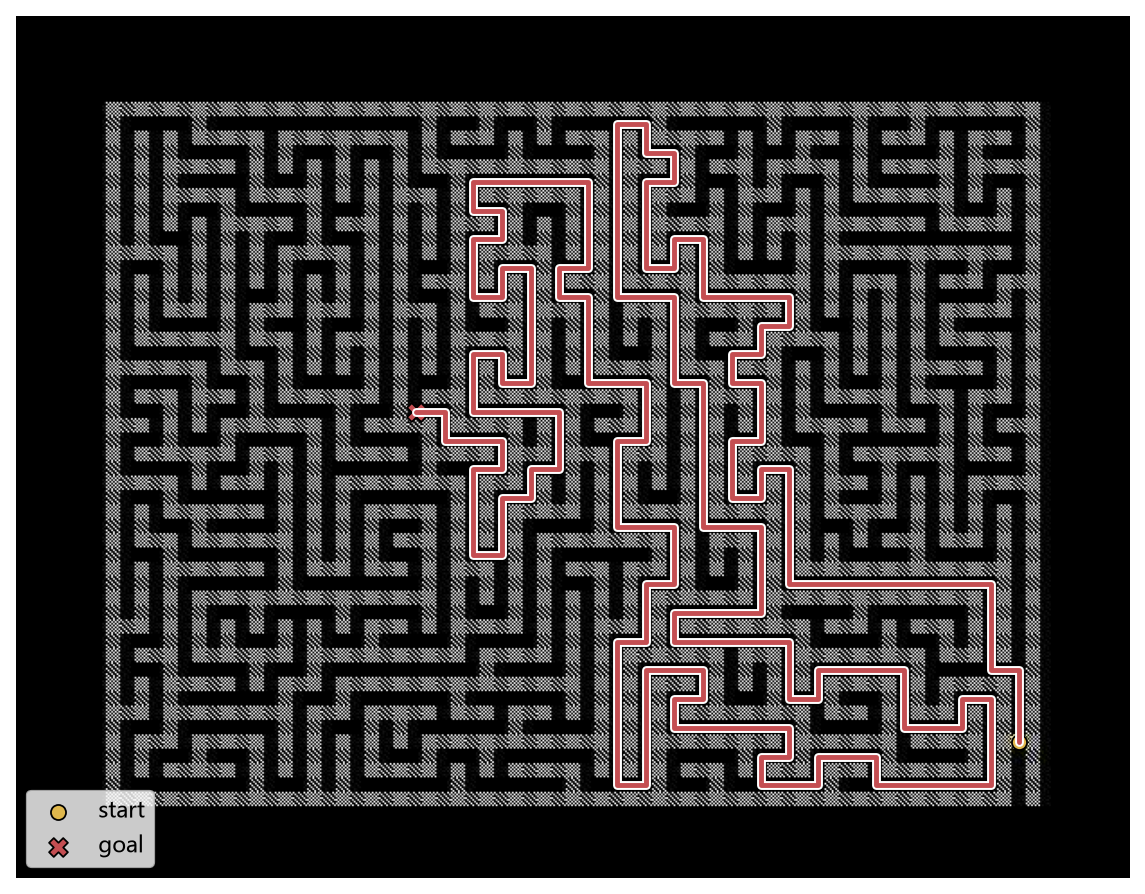
\includegraphics[width=\linewidth]{python/Q7_outputs/random_route_1.png}
        \centerline{(a) 随机终点 1}
    \end{minipage}
    \hfill
    \begin{minipage}{0.48\textwidth}
        \centering
        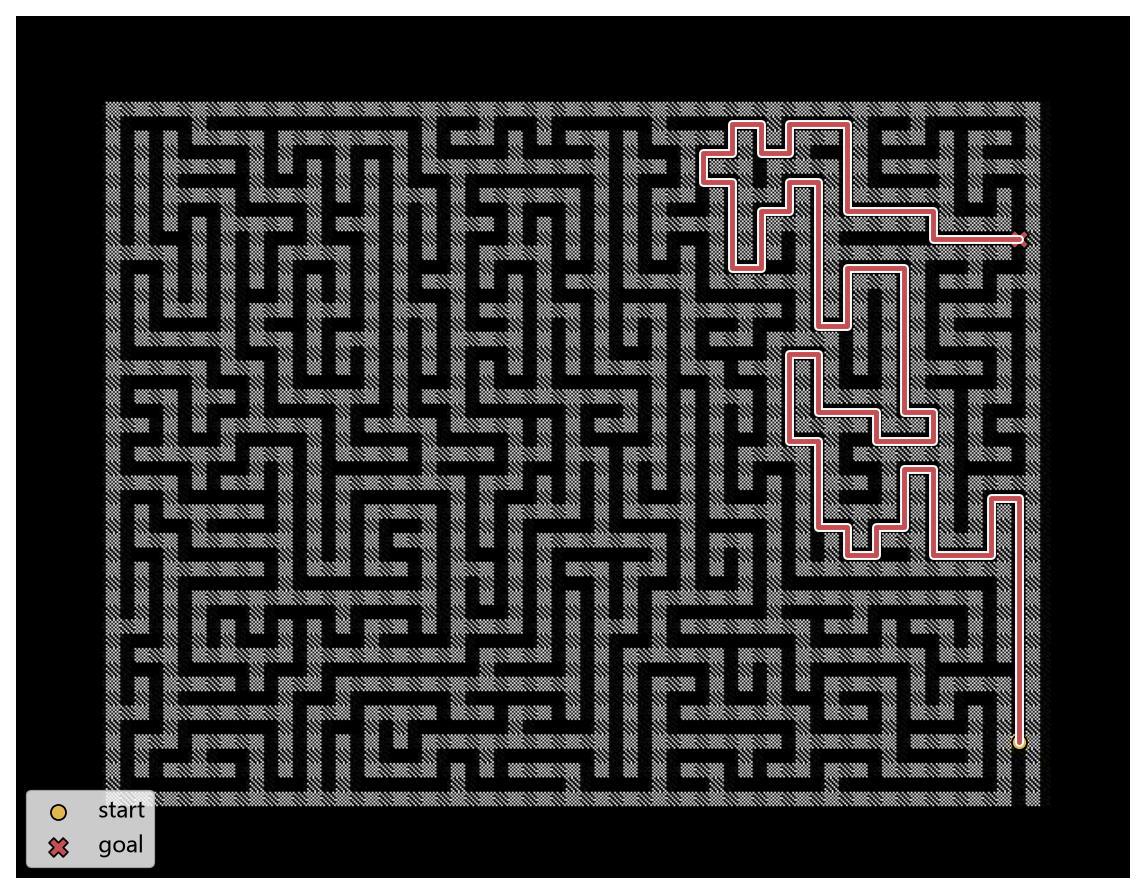
\includegraphics[width=\linewidth]{python/Q7_outputs/random_route_2.png}
        \centerline{(b) 随机终点 2}
    \end{minipage}
    \caption{第7题随机终点路径规划结果}
    \label{fig:q7_random_routes}
\end{figure}

从图中可以看出,  随机终点位于不同位置时,  程序均能在避开墙体的前提下给出从黄色起点到红色终点的可行路线.由于每一步奖励均为 \(-1\),  路径提取阶段沿价值最大的相邻格前进,  对应的就是到目标格的最短路径.

\newpage
\bibliographystyle{plain}
\bibliography{references}

\end{document}



